\section{Modeling the inverter}
\label{invertermodel}

The simulation of an uncontrolled single-phase full bridge inverter (as it was described in \secref{inverter}) was carried out in MATLAB Simulink with LC filtering and with both pure resistive and inductive loads. However, the control system consists of several subsystems which includes voltage and current control, grid synchronization with Phase Locked Loop(PLL), and the strategy of SPWM control on the inverter. Due to the lack of data from the inverter it was reasonable to use measurements from the provided inverter and thus approximate the parameters by that. 

The measurement journal can be found in \secref{app:inverter_step_test} and the test results can be seen in \figref{fig:inverter_data_main}. 

\begin{figure}[H]
\centering
% This file was created by matlab2tikz.

% The latest updates can be retrieved from
%  http://www.mathworks.com/matlabcentral/fileexchange/22022-matlab2tikz-matlab2tikz
% where you can also make suggestions and rate matlab2tikz.

\definecolor{mycolor1}{rgb}{0.00000,0.44700,0.74100}%
\definecolor{mycolor2}{rgb}{0.85000,0.32500,0.09800}%
\definecolor{mycolor3}{rgb}{0.92900,0.69400,0.12500}%
\definecolor{mycolor4}{rgb}{0.49400,0.18400,0.55600}%
\definecolor{mycolor5}{rgb}{0.46600,0.67400,0.18800}%
\definecolor{mycolor6}{rgb}{0.30100,0.74500,0.93300}%

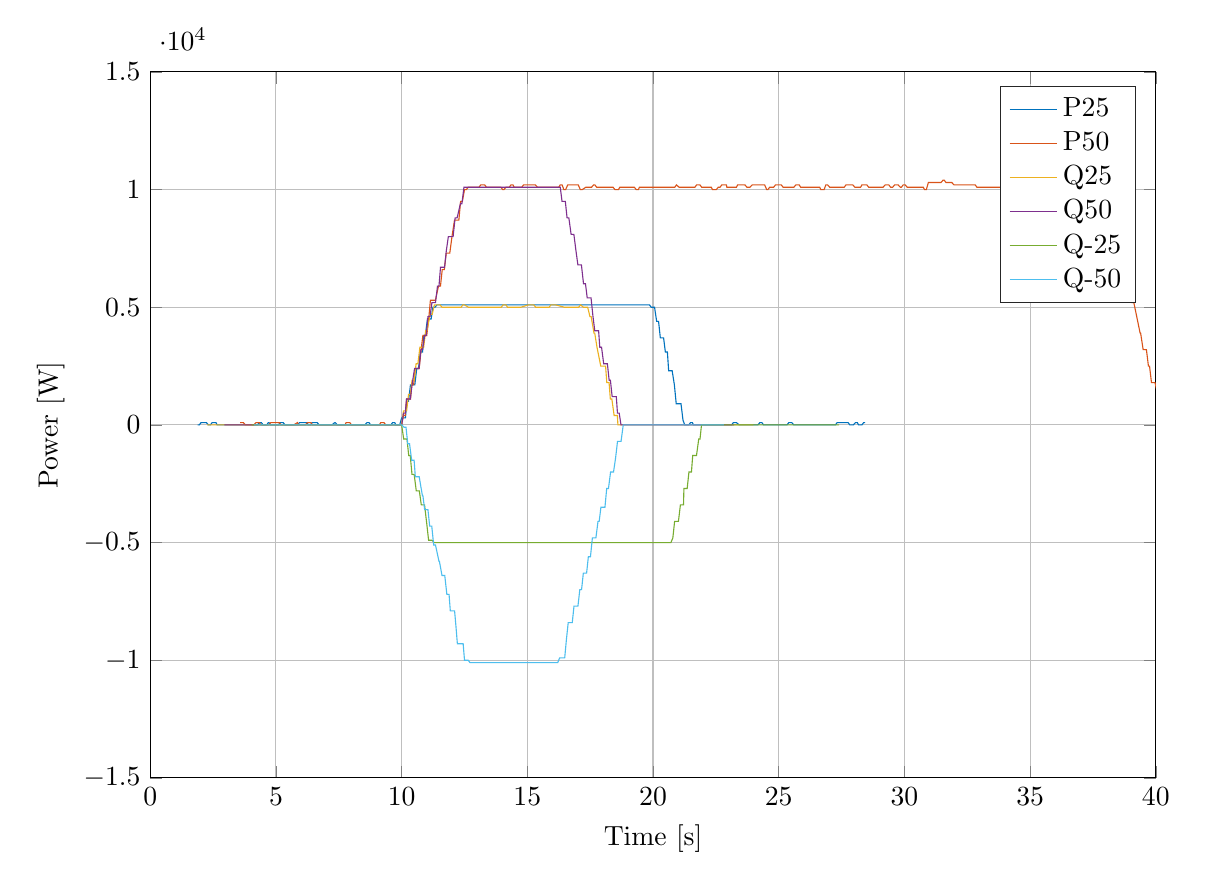
\begin{tikzpicture}

\begin{axis}[%
width=5.028in,
height=3.53in,
at={(1.85in,0.746in)},
scale only axis,
xmin=0,
xmax=40,
xlabel={Time [s]},
xmajorgrids,
ymin=-15000,
ymax=15000,
ylabel={Power [W]},
ymajorgrids,
axis background/.style={fill=white},
legend style={legend cell align=left,align=left,draw=white!15!black}
]
\addplot [color=mycolor1,solid]
 table[row sep=crcr]{%
1.882	0\\
1.952	0\\
2.022	100\\
2.102	100\\
2.162	100\\
2.232	100\\
2.318	0\\
2.393	0\\
2.463	100\\
2.532	100\\
2.616	100\\
2.663	0\\
2.733	0\\
2.816	0\\
2.893	0\\
2.964	0\\
3.033	0\\
3.083	0\\
3.163	0\\
3.233	0\\
3.317	0\\
3.394	0\\
3.464	0\\
3.535	0\\
3.585	0\\
3.665	0\\
3.735	0\\
3.82	0\\
3.865	0\\
3.935	0\\
4.055	0\\
4.075	0\\
4.145	0\\
4.195	0\\
4.266	0\\
4.336	100\\
4.419	100\\
4.495	0\\
4.636	0\\
4.696	100\\
4.722	100\\
4.796	0\\
4.876	0\\
4.956	0\\
5.006	0\\
5.096	0\\
5.166	100\\
5.236	100\\
5.286	100\\
5.367	0\\
5.437	0\\
5.521	0\\
5.597	0\\
5.677	0\\
5.721	0\\
5.797	0\\
5.868	0\\
5.937	100\\
6.019	100\\
6.097	100\\
6.167	100\\
6.238	100\\
6.288	0\\
6.368	0\\
6.438	100\\
6.522	100\\
6.578	100\\
6.639	100\\
6.725	0\\
6.799	0\\
6.869	0\\
6.939	0\\
7.021	0\\
7.07	0\\
7.14	0\\
7.225	0\\
7.34	100\\
7.36	100\\
7.44	0\\
7.49	0\\
7.57	0\\
7.65	0\\
7.7	0\\
7.77	0\\
7.823	0\\
7.9	0\\
7.97	0\\
8.04	0\\
8.123	0\\
8.2	0\\
8.27	0\\
8.324	0\\
8.4	0\\
8.47	0\\
8.54	0\\
8.623	100\\
8.7	100\\
8.77	0\\
8.84	0\\
8.922	0\\
9	0\\
9.07	0\\
9.14	0\\
9.223	0\\
9.27	0\\
9.34	0\\
9.423	0\\
9.5	0\\
9.571	0\\
9.641	100\\
9.724	100\\
9.771	0\\
9.841	0\\
9.923	0\\
10.001	300\\
10.071	300\\
10.151	300\\
10.211	1000\\
10.272	1000\\
10.351	1700\\
10.401	1700\\
10.471	1700\\
10.524	1700\\
10.602	2400\\
10.671	2400\\
10.742	3100\\
10.832	3100\\
10.882	3800\\
10.942	3800\\
11.025	4500\\
11.102	4500\\
11.173	4500\\
11.243	5000\\
11.326	5000\\
11.403	5100\\
11.472	5100\\
11.528	5100\\
11.603	5100\\
11.673	5100\\
11.726	5100\\
11.803	5100\\
11.932	5100\\
11.943	5100\\
12.029	5100\\
12.103	5100\\
12.173	5100\\
12.227	5100\\
12.304	5100\\
12.374	5100\\
12.444	5100\\
12.528	5100\\
12.604	5100\\
12.674	5100\\
12.728	5100\\
12.805	5100\\
12.875	5100\\
12.944	5100\\
13.027	5100\\
13.105	5100\\
13.175	5100\\
13.228	5100\\
13.305	5100\\
13.376	5100\\
13.429	5100\\
13.507	5100\\
13.577	5100\\
13.646	5100\\
13.729	5100\\
13.807	5100\\
13.877	5100\\
13.934	5100\\
14.008	5100\\
14.077	5100\\
14.147	5100\\
14.23	5100\\
14.307	5100\\
14.377	5100\\
14.431	5100\\
14.518	5100\\
14.578	5100\\
14.718	5100\\
14.732	5100\\
14.809	5100\\
14.879	5100\\
14.949	5100\\
15.034	5100\\
15.11	5100\\
15.179	5100\\
15.25	5100\\
15.332	5100\\
15.379	5100\\
15.449	5100\\
15.532	5100\\
15.609	5100\\
15.68	5100\\
15.75	5100\\
15.837	5100\\
15.881	5100\\
15.95	5100\\
16.034	5100\\
16.11	5100\\
16.181	5100\\
16.252	5100\\
16.302	5100\\
16.382	5100\\
16.452	5100\\
16.535	5100\\
16.582	5100\\
16.652	5100\\
16.735	5100\\
16.813	5100\\
16.893	5100\\
16.937	5100\\
17.013	5100\\
17.083	5100\\
17.153	5100\\
17.223	5100\\
17.323	5100\\
17.384	5100\\
17.455	5100\\
17.505	5100\\
17.575	5100\\
17.656	5100\\
17.738	5100\\
17.786	5100\\
17.856	5100\\
17.94	5100\\
18.027	5100\\
18.087	5100\\
18.157	5100\\
18.207	5100\\
18.278	5100\\
18.358	5100\\
18.441	5100\\
18.488	5100\\
18.558	5100\\
18.641	5100\\
18.718	5100\\
18.788	5100\\
18.858	5100\\
18.944	5100\\
18.989	5100\\
19.058	5100\\
19.142	5100\\
19.219	5100\\
19.289	5100\\
19.359	5100\\
19.444	5100\\
19.489	5100\\
19.559	5100\\
19.642	5100\\
19.719	5100\\
19.789	5100\\
19.859	5100\\
19.929	5000\\
19.99	5000\\
20.06	5000\\
20.144	4400\\
20.22	4400\\
20.29	3700\\
20.4	3700\\
20.42	3700\\
20.49	3100\\
20.571	3100\\
20.621	2300\\
20.691	2300\\
20.761	2300\\
20.849	1700\\
20.922	900\\
20.992	900\\
21.062	900\\
21.112	900\\
21.192	200\\
21.262	0\\
21.348	0\\
21.422	0\\
21.492	100\\
21.562	100\\
21.613	0\\
21.683	0\\
21.763	0\\
21.848	0\\
21.923	0\\
21.993	0\\
22.064	0\\
22.114	0\\
22.184	0\\
22.264	0\\
22.35	0\\
22.394	0\\
22.464	0\\
22.547	0\\
22.634	0\\
22.674	0\\
22.748	0\\
22.824	0\\
22.895	0\\
22.965	0\\
23.047	0\\
23.125	0\\
23.195	100\\
23.266	100\\
23.316	100\\
23.425	0\\
23.457	0\\
23.537	0\\
23.597	0\\
23.668	0\\
23.752	0\\
23.828	0\\
23.898	0\\
23.968	0\\
24.05	0\\
24.098	0\\
24.168	0\\
24.25	100\\
24.328	100\\
24.398	0\\
24.468	0\\
24.518	0\\
24.598	0\\
24.669	0\\
24.752	0\\
24.829	0\\
24.898	0\\
24.968	0\\
25.018	0\\
25.099	0\\
25.169	0\\
25.252	0\\
25.329	0\\
25.399	100\\
25.469	100\\
25.519	100\\
25.599	0\\
25.669	0\\
25.752	0\\
25.819	0\\
25.86	0\\
25.94	0\\
26	0\\
26.055	0\\
26.13	0\\
26.2	0\\
26.27	0\\
26.34	0\\
26.421	0\\
26.471	0\\
26.556	0\\
26.632	0\\
26.692	0\\
26.755	0\\
26.822	0\\
26.902	0\\
26.962	0\\
27.054	0\\
27.123	0\\
27.203	0\\
27.257	0\\
27.323	100\\
27.404	100\\
27.458	100\\
27.524	100\\
27.605	100\\
27.675	100\\
27.759	100\\
27.825	0\\
27.905	0\\
27.966	0\\
28.057	100\\
28.126	100\\
28.176	0\\
28.246	0\\
28.307	0\\
28.377	100\\
28.437	100\\
};
\addlegendentry{P25};

\addplot [color=mycolor2,solid]
 table[row sep=crcr]{%
3.573	100\\
3.634	100\\
3.704	100\\
3.785	0\\
3.874	0\\
3.934	0\\
4.005	0\\
4.055	0\\
4.126	0\\
4.205	100\\
4.289	100\\
4.336	100\\
4.406	0\\
4.489	0\\
4.566	0\\
4.636	0\\
4.706	0\\
4.796	100\\
4.846	100\\
4.906	100\\
4.989	100\\
5.066	100\\
5.136	100\\
5.206	0\\
5.294	0\\
5.337	0\\
5.407	0\\
5.49	0\\
5.567	0\\
5.637	0\\
5.707	0\\
5.857	100\\
5.892	0\\
5.957	0\\
6.007	0\\
6.09	0\\
6.167	0\\
6.257	100\\
6.307	100\\
6.39	100\\
6.457	0\\
6.527	0\\
6.598	0\\
6.678	0\\
6.738	0\\
6.808	0\\
6.891	0\\
6.968	0\\
7.038	0\\
7.093	0\\
7.168	0\\
7.238	0\\
7.308	0\\
7.392	0\\
7.458	0\\
7.548	0\\
7.638	0\\
7.658	0\\
7.748	0\\
7.792	100\\
7.868	100\\
7.938	100\\
8.008	0\\
8.092	0\\
8.168	0\\
8.238	0\\
8.291	0\\
8.369	0\\
8.439	0\\
8.509	0\\
8.591	0\\
8.669	0\\
8.739	0\\
8.792	0\\
8.869	0\\
8.94	0\\
9.01	0\\
9.111	0\\
9.17	100\\
9.211	100\\
9.294	100\\
9.372	0\\
9.452	0\\
9.496	0\\
9.572	0\\
9.653	0\\
9.696	0\\
9.773	0\\
9.843	0\\
9.914	0\\
9.997	0\\
10.074	400\\
10.144	400\\
10.197	1100\\
10.274	1100\\
10.355	1100\\
10.399	1700\\
10.475	1700\\
10.545	2400\\
10.615	2400\\
10.698	2400\\
10.776	3200\\
10.845	3800\\
10.915	3800\\
10.999	3800\\
11.076	4500\\
11.145	5300\\
11.199	5300\\
11.276	5300\\
11.345	5300\\
11.466	5900\\
11.475	5900\\
11.545	5900\\
11.615	6600\\
11.698	6600\\
11.775	7300\\
11.845	7300\\
11.915	7300\\
12.002	8000\\
12.103	8700\\
12.146	8700\\
12.199	8700\\
12.276	8700\\
12.346	9500\\
12.416	9500\\
12.501	10000\\
12.576	10000\\
12.646	10100\\
12.699	10100\\
12.776	10100\\
12.846	10100\\
12.917	10100\\
13	10100\\
13.077	10100\\
13.147	10200\\
13.217	10200\\
13.302	10200\\
13.377	10100\\
13.447	10100\\
13.517	10100\\
13.605	10100\\
13.647	10100\\
13.717	10100\\
13.803	10100\\
13.878	10100\\
13.948	10100\\
14.018	10000\\
14.068	10000\\
14.149	10100\\
14.202	10100\\
14.279	10100\\
14.349	10200\\
14.429	10200\\
14.479	10100\\
14.549	10100\\
14.619	10100\\
14.702	10100\\
14.78	10100\\
14.85	10200\\
14.92	10200\\
15.003	10200\\
15.15	10200\\
15.18	10200\\
15.251	10200\\
15.321	10200\\
15.403	10100\\
15.481	10100\\
15.541	10100\\
15.612	10100\\
15.692	10100\\
15.752	10100\\
15.821	10100\\
15.904	10100\\
15.982	10100\\
16.052	10100\\
16.104	10100\\
16.182	10100\\
16.252	10100\\
16.306	10200\\
16.383	10200\\
16.453	10000\\
16.524	10000\\
16.606	10200\\
16.683	10200\\
16.754	10200\\
16.808	10200\\
16.884	10200\\
16.955	10200\\
17.025	10200\\
17.108	10000\\
17.185	10000\\
17.325	10100\\
17.345	10100\\
17.413	10100\\
17.486	10100\\
17.555	10100\\
17.636	10200\\
17.686	10200\\
17.756	10100\\
17.826	10100\\
17.91	10100\\
17.986	10100\\
18.066	10100\\
18.11	10100\\
18.186	10100\\
18.256	10100\\
18.326	10100\\
18.41	10100\\
18.487	10000\\
18.557	10000\\
18.627	10000\\
18.677	10100\\
18.748	10100\\
18.818	10100\\
18.898	10100\\
18.959	10100\\
19.029	10100\\
19.114	10100\\
19.189	10100\\
19.259	10100\\
19.33	10000\\
19.416	10000\\
19.46	10100\\
19.53	10100\\
19.614	10100\\
19.69	10100\\
19.771	10100\\
19.821	10100\\
19.915	10100\\
19.961	10100\\
20.041	10100\\
20.101	10100\\
20.182	10100\\
20.223	10100\\
20.303	10100\\
20.393	10100\\
20.463	10100\\
20.544	10100\\
20.617	10100\\
20.674	10100\\
20.722	10100\\
20.794	10100\\
20.864	10100\\
20.934	10200\\
21.034	10100\\
21.094	10100\\
21.164	10100\\
21.244	10100\\
21.345	10100\\
21.365	10100\\
21.434	10100\\
21.523	10100\\
21.595	10100\\
21.665	10100\\
21.734	10200\\
21.818	10200\\
21.865	10200\\
21.935	10100\\
22.018	10100\\
22.085	10100\\
22.165	10100\\
22.235	10100\\
22.318	10100\\
22.365	10000\\
22.435	10000\\
22.518	10000\\
22.594	10100\\
22.665	10100\\
22.735	10200\\
22.819	10200\\
22.919	10200\\
22.936	10100\\
23.02	10100\\
23.096	10100\\
23.166	10100\\
23.236	10100\\
23.318	10100\\
23.366	10200\\
23.435	10200\\
23.519	10200\\
23.635	10200\\
23.655	10200\\
23.736	10100\\
23.786	10100\\
23.856	10100\\
23.946	10200\\
23.996	10200\\
24.067	10200\\
24.137	10200\\
24.221	10200\\
24.298	10200\\
24.368	10200\\
24.439	10200\\
24.522	10000\\
24.568	10000\\
24.639	10100\\
24.722	10100\\
24.799	10100\\
24.87	10200\\
24.941	10200\\
25.023	10200\\
25.101	10200\\
25.172	10100\\
25.242	10100\\
25.325	10100\\
25.402	10100\\
25.472	10100\\
25.528	10100\\
25.602	10100\\
25.682	10200\\
25.728	10200\\
25.813	10200\\
25.873	10100\\
25.943	10100\\
26.027	10100\\
26.104	10100\\
26.173	10100\\
26.229	10100\\
26.304	10100\\
26.373	10100\\
26.443	10100\\
26.528	10100\\
26.628	10100\\
26.674	10000\\
26.73	10000\\
26.804	10000\\
26.874	10200\\
26.944	10200\\
27.027	10100\\
27.104	10100\\
27.174	10100\\
27.23	10100\\
27.305	10100\\
27.375	10100\\
27.445	10100\\
27.532	10100\\
27.605	10100\\
27.675	10200\\
27.728	10200\\
27.805	10200\\
27.875	10200\\
27.945	10200\\
28.028	10100\\
28.106	10100\\
28.176	10100\\
28.257	10100\\
28.306	10200\\
28.376	10200\\
28.431	10200\\
28.506	10200\\
28.577	10100\\
28.647	10100\\
28.732	10100\\
28.807	10100\\
28.877	10100\\
28.931	10100\\
29.008	10100\\
29.078	10100\\
29.149	10100\\
29.235	10200\\
29.308	10200\\
29.379	10200\\
29.449	10100\\
29.532	10100\\
29.609	10200\\
29.679	10200\\
29.749	10200\\
29.837	10100\\
29.88	10100\\
29.949	10200\\
30.032	10200\\
30.109	10100\\
30.18	10100\\
30.25	10100\\
30.333	10100\\
30.38	10100\\
30.45	10100\\
30.534	10100\\
30.61	10100\\
30.68	10100\\
30.751	10100\\
30.8	10000\\
30.871	10000\\
30.951	10300\\
31.034	10300\\
31.082	10300\\
31.152	10300\\
31.235	10300\\
31.312	10300\\
31.382	10300\\
31.453	10300\\
31.535	10400\\
31.583	10400\\
31.653	10300\\
31.739	10300\\
31.813	10300\\
31.883	10300\\
31.973	10200\\
32.023	10200\\
32.083	10200\\
32.153	10200\\
32.237	10200\\
32.313	10200\\
32.383	10200\\
32.453	10200\\
32.503	10200\\
32.583	10200\\
32.653	10200\\
32.737	10200\\
32.814	10200\\
32.883	10100\\
32.954	10100\\
33.004	10100\\
33.083	10100\\
33.154	10100\\
33.237	10100\\
33.314	10100\\
33.434	10100\\
33.454	10100\\
33.504	10100\\
33.584	10100\\
33.654	10100\\
33.739	10100\\
33.785	10100\\
33.854	10100\\
33.939	10100\\
34.015	10100\\
34.085	10100\\
34.155	10100\\
34.245	10100\\
34.295	10100\\
34.439	10100\\
34.456	10100\\
34.538	10100\\
34.617	10100\\
34.687	10100\\
34.757	10100\\
34.84	10100\\
34.907	10100\\
34.987	10100\\
35.04	10100\\
35.117	10100\\
35.187	10100\\
35.24	10100\\
35.317	10100\\
35.387	10100\\
35.458	10100\\
35.54	10100\\
35.618	10100\\
35.688	10100\\
35.741	10100\\
35.818	10100\\
35.888	10100\\
35.958	10100\\
36.045	10100\\
36.118	10100\\
36.189	10100\\
36.245	10100\\
36.319	10100\\
36.442	10100\\
36.459	10100\\
36.543	10100\\
36.649	10100\\
36.699	10100\\
36.759	10100\\
36.848	10100\\
36.919	10100\\
36.99	10100\\
37.061	10100\\
37.151	10100\\
37.201	10100\\
37.261	10100\\
37.344	10100\\
37.422	10100\\
37.491	10100\\
37.562	10100\\
37.646	10100\\
37.692	10100\\
37.762	10100\\
37.846	10100\\
37.922	10100\\
37.992	9600\\
38.062	9600\\
38.112	9600\\
38.192	8900\\
38.263	8900\\
38.346	8000\\
38.422	8000\\
38.493	7500\\
38.603	7500\\
38.623	7500\\
38.693	6700\\
38.763	6700\\
38.848	5900\\
38.894	5900\\
38.964	5900\\
39.05	5200\\
39.124	5200\\
39.375	3900\\
39.395	3900\\
39.495	3200\\
39.549	3200\\
39.625	3200\\
39.705	2500\\
39.749	2500\\
39.826	1800\\
39.896	1800\\
39.966	1800\\
40.287	300\\
40.327	300\\
40.438	0\\
40.457	0\\
40.618	0\\
40.638	0\\
40.928	0\\
40.954	0\\
41.109	0\\
41.109	0\\
41.152	0\\
41.239	0\\
41.558	0\\
41.58	0\\
41.68	0\\
41.71	0\\
41.757	100\\
41.831	100\\
41.901	100\\
41.982	0\\
42.055	0\\
42.131	0\\
42.201	0\\
42.491	0\\
42.511	0\\
42.621	0\\
42.641	0\\
42.701	0\\
42.812	100\\
42.832	100\\
43.121	0\\
43.141	0\\
43.254	0\\
43.271	0\\
43.356	0\\
43.431	0\\
43.501	0\\
43.553	0\\
43.632	0\\
43.701	0\\
43.771	0\\
44.061	0\\
44.072	0\\
44.154	100\\
44.232	100\\
44.302	100\\
44.372	0\\
44.457	0\\
44.542	0\\
44.572	0\\
44.654	0\\
44.732	0\\
44.802	0\\
44.872	0\\
44.956	0\\
45.002	0\\
45.073	0\\
45.156	0\\
45.232	0\\
45.303	0\\
45.372	0\\
45.453	0\\
45.502	0\\
45.573	0\\
45.655	0\\
45.732	0\\
45.802	0\\
45.872	0\\
45.955	100\\
46.003	100\\
46.073	0\\
46.156	0\\
46.233	100\\
46.303	100\\
46.383	100\\
46.433	100\\
46.504	100\\
46.574	0\\
46.657	0\\
46.734	100\\
46.804	100\\
46.874	100\\
46.924	0\\
46.994	0\\
47.074	0\\
47.158	0\\
47.204	0\\
47.275	100\\
47.345	100\\
47.434	0\\
47.495	0\\
47.557	0\\
47.658	0\\
47.734	0\\
47.805	0\\
47.874	0\\
47.934	100\\
48.057	100\\
48.095	0\\
48.159	0\\
48.225	0\\
48.305	0\\
48.365	0\\
48.425	0\\
48.506	0\\
48.566	0\\
48.627	0\\
48.706	0\\
48.777	0\\
48.847	0\\
};
\addlegendentry{P50};

\addplot [color=mycolor3,solid]
 table[row sep=crcr]{%
2.264	0\\
2.334	0\\
2.404	0\\
2.487	0\\
2.564	0\\
2.634	0\\
2.704	0\\
2.789	0\\
2.864	0\\
2.934	0\\
2.992	0\\
3.065	0\\
3.135	0\\
3.205	0\\
3.288	0\\
3.365	0\\
3.435	0\\
3.788	0\\
3.805	0\\
3.889	0\\
3.965	0\\
4.036	0\\
4.106	0\\
4.156	0\\
4.226	0\\
4.297	0\\
4.377	0\\
4.437	0\\
4.508	0\\
4.591	0\\
4.668	0\\
4.738	0\\
4.808	0\\
4.878	0\\
4.939	0\\
5.009	0\\
5.092	0\\
5.139	0\\
5.209	0\\
5.291	0\\
5.369	0\\
5.439	0\\
5.51	0\\
5.593	0\\
5.64	0\\
5.711	0\\
5.794	0\\
5.871	0\\
5.941	0\\
6.011	0\\
6.061	0\\
6.131	0\\
6.202	0\\
6.282	0\\
6.372	0\\
6.442	0\\
6.512	0\\
6.562	0\\
6.662	0\\
6.722	0\\
6.772	0\\
6.852	0\\
6.912	0\\
6.995	0\\
7.072	0\\
7.193	0\\
7.222	0\\
7.272	0\\
7.343	0\\
7.412	0\\
7.495	0\\
7.572	0\\
7.643	0\\
7.713	0\\
7.798	0\\
7.843	0\\
7.913	0\\
7.996	0\\
8.073	0\\
8.143	0\\
8.213	0\\
8.295	0\\
8.343	0\\
8.413	0\\
8.497	0\\
8.574	0\\
8.644	0\\
8.714	0\\
8.797	0\\
8.844	0\\
8.914	0\\
8.997	0\\
9.074	0\\
9.144	0\\
9.214	0\\
9.264	0\\
9.334	0\\
9.414	0\\
9.499	0\\
9.574	0\\
9.644	0\\
9.715	0\\
9.765	0\\
9.844	0\\
9.915	0\\
9.998	0\\
10.075	600\\
10.154	600\\
10.199	600\\
10.275	1300\\
10.345	1300\\
10.415	1900\\
10.498	1900\\
10.575	2600\\
10.646	2600\\
10.726	3300\\
10.806	3300\\
10.876	3300\\
10.956	4000\\
11.006	4000\\
11.136	4700\\
11.156	4700\\
11.216	4700\\
11.303	5100\\
11.386	5100\\
11.477	5100\\
11.527	5100\\
11.607	5000\\
11.677	5000\\
11.717	5000\\
11.804	5000\\
11.877	5000\\
11.958	5000\\
12.008	5000\\
12.101	5000\\
12.158	5000\\
12.208	5000\\
12.301	5000\\
12.369	5000\\
12.429	5100\\
12.499	5100\\
12.659	5000\\
12.689	5000\\
12.77	5000\\
12.82	5000\\
12.903	5000\\
12.98	5000\\
13.131	5000\\
13.161	5000\\
13.221	5000\\
13.311	5000\\
13.371	5000\\
13.412	5000\\
13.492	5000\\
13.562	5000\\
13.611	5000\\
13.704	5000\\
13.752	5000\\
13.832	5000\\
13.892	5000\\
13.963	5000\\
14.033	5100\\
14.093	5100\\
14.152	5100\\
14.213	5000\\
14.363	5000\\
14.393	5000\\
14.453	5000\\
14.534	5000\\
14.594	5000\\
14.674	5000\\
14.734	5000\\
15.045	5100\\
15.075	5100\\
15.115	5100\\
15.195	5100\\
15.255	5100\\
15.335	5000\\
15.416	5000\\
15.496	5000\\
15.556	5000\\
15.626	5000\\
15.71	5000\\
15.787	5000\\
15.867	5000\\
15.937	5100\\
16.007	5100\\
16.067	5100\\
16.127	5100\\
16.478	5000\\
16.498	5000\\
16.589	5000\\
16.659	5000\\
16.889	5000\\
16.919	5000\\
16.979	5000\\
17.039	5000\\
17.12	5100\\
17.23	5000\\
17.25	5000\\
17.32	5000\\
17.4	5000\\
17.491	4600\\
17.54	4600\\
17.651	3900\\
17.681	3900\\
17.771	3300\\
17.921	2500\\
17.961	2500\\
18.081	2500\\
18.112	2500\\
18.161	1800\\
18.251	1800\\
18.301	1100\\
18.362	1100\\
18.452	400\\
18.582	400\\
18.602	0\\
18.672	0\\
18.72	0\\
18.802	0\\
18.862	0\\
18.952	0\\
19.002	0\\
19.072	0\\
19.133	0\\
19.22	0\\
19.303	0\\
19.363	0\\
19.432	0\\
19.52	0\\
19.573	0\\
19.663	0\\
19.742	0\\
19.792	0\\
19.862	0\\
19.942	0\\
19.992	0\\
20.072	0\\
20.142	0\\
20.202	0\\
20.282	0\\
20.362	0\\
20.432	0\\
20.492	0\\
20.532	0\\
20.617	0\\
20.682	0\\
20.723	0\\
20.803	0\\
20.923	0\\
20.943	0\\
21.023	0\\
21.123	0\\
21.183	0\\
21.223	0\\
21.323	0\\
21.374	0\\
21.434	0\\
21.574	0\\
21.614	0\\
21.674	0\\
21.734	0\\
21.794	0\\
21.874	0\\
21.923	0\\
22.015	0\\
22.065	0\\
22.146	0\\
22.196	0\\
22.275	0\\
22.345	0\\
22.405	0\\
22.465	0\\
22.525	0\\
22.62	0\\
22.676	0\\
22.723	0\\
22.821	0\\
22.921	0\\
23.127	0\\
23.157	0\\
23.22	0\\
23.276	0\\
23.376	0\\
23.437	0\\
23.518	0\\
23.597	0\\
23.637	0\\
23.737	0\\
23.797	0\\
23.867	0\\
23.927	0\\
23.987	0\\
};
\addlegendentry{Q25};

\addplot [color=mycolor4,solid]
 table[row sep=crcr]{%
2.952	0\\
3.023	0\\
3.103	0\\
3.163	0\\
3.234	0\\
3.319	0\\
3.394	0\\
3.465	0\\
3.526	0\\
3.606	0\\
3.665	0\\
3.735	0\\
3.82	0\\
3.896	0\\
3.966	0\\
4.036	0\\
4.086	0\\
4.166	0\\
4.237	0\\
4.32	0\\
4.367	0\\
4.437	0\\
4.521	0\\
4.598	0\\
4.668	0\\
4.738	0\\
4.822	0\\
4.888	0\\
4.938	0\\
5.028	0\\
5.078	0\\
5.138	0\\
5.221	0\\
5.299	0\\
5.368	0\\
5.439	0\\
5.522	0\\
5.599	0\\
5.669	0\\
5.739	0\\
5.789	0\\
5.86	0\\
5.939	0\\
6.021	0\\
6.07	0\\
6.139	0\\
6.227	0\\
6.3	0\\
6.37	0\\
6.439	0\\
6.522	0\\
6.569	0\\
6.639	0\\
6.722	0\\
6.799	0\\
6.87	0\\
6.939	0\\
7.024	0\\
7.07	0\\
7.14	0\\
7.223	0\\
7.3	0\\
7.371	0\\
7.441	0\\
7.524	0\\
7.57	0\\
7.641	0\\
7.724	0\\
7.8	0\\
7.87	0\\
7.941	0\\
8.024	0\\
8.071	0\\
8.141	0\\
8.224	0\\
8.301	0\\
8.371	0\\
8.441	0\\
8.491	0\\
8.562	0\\
8.642	0\\
8.724	0\\
8.802	0\\
8.883	0\\
8.93	0\\
9.002	0\\
9.073	0\\
9.143	0\\
9.226	0\\
9.273	0\\
9.343	0\\
9.429	0\\
9.503	0\\
9.574	0\\
9.644	0\\
9.727	0\\
9.774	0\\
9.844	0\\
9.927	0\\
10.004	0\\
10.074	500\\
10.144	500\\
10.194	1100\\
10.265	1100\\
10.344	1100\\
10.427	1800\\
10.515	2400\\
10.575	2400\\
10.645	2400\\
10.695	2400\\
10.765	3200\\
10.835	3200\\
10.916	3800\\
10.976	3800\\
11.046	4600\\
11.127	4600\\
11.205	5200\\
11.276	5200\\
11.346	5200\\
11.427	5900\\
11.486	5900\\
11.546	6700\\
11.628	6700\\
11.707	6700\\
11.777	7400\\
11.857	8000\\
11.907	8000\\
11.987	8000\\
12.047	8000\\
12.128	8800\\
12.207	8800\\
12.337	9400\\
12.347	9400\\
12.397	9400\\
12.478	10100\\
12.548	10100\\
12.636	10100\\
12.708	10100\\
12.778	10100\\
12.847	10100\\
12.897	10100\\
12.978	10100\\
13.058	10100\\
13.108	10100\\
13.178	10100\\
13.249	10100\\
13.334	10100\\
13.419	10100\\
13.589	10100\\
13.599	10100\\
13.648	10100\\
13.737	10100\\
13.809	10100\\
13.879	10100\\
13.935	10100\\
14.009	10100\\
14.079	10100\\
14.149	10100\\
14.233	10100\\
14.309	10100\\
14.399	10100\\
14.439	10100\\
14.537	10100\\
14.579	10100\\
14.649	10100\\
14.732	10100\\
14.809	10100\\
14.879	10100\\
14.933	10100\\
15.009	10100\\
15.09	10100\\
15.132	10100\\
15.21	10100\\
15.28	10100\\
15.35	10100\\
15.44	10100\\
15.52	10100\\
15.579	10100\\
15.649	10100\\
15.732	10100\\
15.809	10100\\
15.88	10100\\
15.933	10100\\
16.009	10100\\
16.08	10100\\
16.15	10100\\
16.235	10100\\
16.31	10100\\
16.38	9500\\
16.433	9500\\
16.511	9500\\
16.58	8800\\
16.651	8800\\
16.741	8100\\
16.791	8100\\
16.851	8100\\
16.934	7400\\
17.011	6800\\
17.081	6800\\
17.151	6800\\
17.235	6000\\
17.312	6000\\
17.382	5400\\
17.452	5400\\
17.534	5400\\
17.612	4600\\
17.682	4000\\
17.752	4000\\
17.835	4000\\
17.882	3300\\
17.952	3300\\
18.037	2600\\
18.113	2600\\
18.184	2600\\
18.254	1900\\
18.304	1900\\
18.374	1200\\
18.454	1200\\
18.539	1200\\
18.585	500\\
18.655	500\\
18.725	0\\
18.786	0\\
18.841	0\\
18.915	0\\
18.986	0\\
19.056	0\\
19.14	0\\
19.216	0\\
19.286	0\\
19.339	0\\
19.416	0\\
19.556	0\\
19.556	0\\
19.64	0\\
19.717	0\\
19.787	0\\
19.847	0\\
19.898	0\\
19.968	0\\
20.041	0\\
20.118	0\\
20.189	0\\
20.259	0\\
20.342	0\\
20.419	0\\
20.489	0\\
20.545	0\\
20.619	0\\
20.689	0\\
20.759	0\\
20.843	0\\
20.919	0\\
20.99	0\\
21.045	0\\
21.11	0\\
21.19	0\\
21.244	0\\
21.31	0\\
21.39	0\\
21.444	0\\
21.51	0\\
21.59	0\\
21.647	0\\
21.71	0\\
21.79	0\\
21.845	0\\
21.944	0\\
22.01	0\\
22.09	0\\
22.16	0\\
22.22	0\\
22.29	0\\
22.36	0\\
22.43	0\\
22.52	0\\
22.59	0\\
22.67	0\\
22.71	0\\
22.79	0\\
22.91	0\\
22.943	0\\
23.011	0\\
23.091	0\\
23.161	0\\
23.221	0\\
};
\addlegendentry{Q50};

\addplot [color=mycolor5,solid]
 table[row sep=crcr]{%
4.035	0\\
4.116	0\\
4.176	0\\
4.245	0\\
4.295	0\\
4.385	0\\
4.446	0\\
4.516	0\\
4.566	0\\
4.635	0\\
4.706	0\\
4.776	0\\
4.856	0\\
4.958	0\\
4.978	0\\
5.048	0\\
5.098	0\\
5.178	0\\
5.238	0\\
5.308	0\\
5.358	0\\
5.438	0\\
5.508	0\\
5.59	0\\
5.668	0\\
5.738	0\\
5.808	0\\
5.858	0\\
5.938	0\\
6.008	0\\
6.091	0\\
6.168	0\\
6.238	0\\
6.308	0\\
6.358	0\\
6.428	0\\
6.508	0\\
6.59	0\\
6.668	0\\
6.738	0\\
6.808	0\\
6.858	0\\
6.928	0\\
7.008	0\\
7.092	0\\
7.168	0\\
7.239	0\\
7.308	0\\
7.393	0\\
7.468	0\\
7.538	0\\
7.609	0\\
7.691	0\\
7.769	0\\
7.838	0\\
7.892	0\\
7.969	0\\
8.038	0\\
8.109	0\\
8.193	0\\
8.269	0\\
8.339	0\\
8.393	0\\
8.469	0\\
8.539	0\\
8.609	0\\
8.699	0\\
8.759	0\\
8.839	0\\
8.899	0\\
8.98	0\\
9.04	0\\
9.11	0\\
9.2	0\\
9.251	0\\
9.311	0\\
9.399	0\\
9.471	0\\
9.541	0\\
9.612	0\\
9.693	0\\
9.772	0\\
9.842	0\\
9.912	0\\
10	0\\
10.082	-600\\
10.142	-600\\
10.212	-600\\
10.282	-1300\\
10.342	-1300\\
10.412	-2100\\
10.498	-2100\\
10.582	-2800\\
10.632	-2800\\
10.703	-2800\\
10.783	-3400\\
10.843	-3400\\
10.912	-3400\\
10.999	-4200\\
11.073	-4900\\
11.142	-4900\\
11.212	-4900\\
11.296	-5000\\
11.343	-5000\\
11.413	-5000\\
11.496	-5000\\
11.573	-5000\\
11.643	-5000\\
11.713	-5000\\
11.798	-5000\\
11.844	-5000\\
11.913	-5000\\
11.997	-5000\\
12.074	-5000\\
12.144	-5000\\
12.214	-5000\\
12.264	-5000\\
12.334	-5000\\
12.414	-5000\\
12.497	-5000\\
12.574	-5000\\
12.645	-5000\\
12.715	-5000\\
12.775	-5000\\
12.856	-5000\\
12.965	-5000\\
12.985	-5000\\
13.075	-5000\\
13.115	-5000\\
13.199	-5000\\
13.276	-5000\\
13.346	-5000\\
13.416	-5000\\
13.556	-5000\\
13.556	-5000\\
13.617	-5000\\
13.701	-5000\\
13.777	-5000\\
13.847	-5000\\
13.937	-5000\\
13.987	-5000\\
14.047	-5000\\
14.117	-5000\\
14.201	-5000\\
14.277	-5000\\
14.348	-5000\\
14.418	-5000\\
14.468	-5000\\
14.547	-5000\\
14.618	-5000\\
14.707	-5000\\
14.758	-5000\\
14.818	-5000\\
14.901	-5000\\
14.978	-5000\\
15.048	-5000\\
15.118	-5000\\
15.202	-5000\\
15.248	-5000\\
15.318	-5000\\
15.408	-5000\\
15.458	-5000\\
15.518	-5000\\
15.605	-5000\\
15.678	-5000\\
15.748	-5000\\
15.818	-5000\\
15.906	-5000\\
15.979	-5000\\
16.048	-5000\\
16.129	-5000\\
16.179	-5000\\
16.249	-5000\\
16.319	-5000\\
16.409	-5000\\
16.459	-5000\\
16.519	-5000\\
16.606	-5000\\
16.68	-5000\\
16.749	-5000\\
16.819	-5000\\
16.903	-5000\\
16.98	-5000\\
17.05	-5000\\
17.13	-5000\\
17.18	-5000\\
17.25	-5000\\
17.32	-5000\\
17.408	-5000\\
17.48	-5000\\
17.55	-5000\\
17.62	-5000\\
17.67	-5000\\
17.74	-5000\\
17.89	-5000\\
17.91	-5000\\
17.99	-5000\\
18.051	-5000\\
18.121	-5000\\
18.181	-5000\\
18.251	-5000\\
18.321	-5000\\
18.405	-5000\\
18.451	-5000\\
18.521	-5000\\
18.605	-5000\\
18.681	-5000\\
18.752	-5000\\
18.822	-5000\\
18.912	-5000\\
18.962	-5000\\
19.042	-5000\\
19.112	-5000\\
19.163	-5000\\
19.223	-5000\\
19.306	-5000\\
19.383	-5000\\
19.454	-5000\\
19.524	-5000\\
19.607	-5000\\
19.654	-5000\\
19.725	-5000\\
19.808	-5000\\
19.885	-5000\\
19.955	-5000\\
20.025	-5000\\
20.095	-5000\\
20.156	-5000\\
20.226	-5000\\
20.309	-5000\\
20.386	-5000\\
20.457	-5000\\
20.527	-5000\\
20.577	-5000\\
20.667	-5000\\
20.712	-5000\\
20.788	-4800\\
20.858	-4100\\
20.928	-4100\\
21.01	-4100\\
21.088	-3400\\
21.212	-3400\\
21.228	-2700\\
21.338	-2700\\
21.358	-2700\\
21.428	-2000\\
21.528	-2000\\
21.578	-1300\\
21.658	-1300\\
21.728	-1300\\
21.818	-600\\
21.868	-600\\
21.928	0\\
22.014	0\\
22.098	0\\
22.148	0\\
22.228	0\\
22.312	0\\
22.358	0\\
22.428	0\\
22.512	0\\
22.588	0\\
22.659	0\\
22.729	0\\
22.814	0\\
22.859	0\\
22.929	0\\
23.014	0\\
23.089	0\\
23.179	0\\
23.229	0\\
23.312	0\\
23.359	0\\
23.429	0\\
23.519	0\\
23.569	0\\
23.629	0\\
23.716	0\\
23.8	0\\
23.86	0\\
23.93	0\\
24.013	0\\
24.06	0\\
24.131	0\\
24.214	0\\
24.351	0\\
24.361	0\\
24.431	0\\
24.516	0\\
24.562	0\\
24.632	0\\
24.714	0\\
24.822	0\\
24.863	0\\
24.933	0\\
24.983	0\\
25.053	0\\
25.123	0\\
25.203	0\\
25.264	0\\
25.334	0\\
25.417	0\\
25.494	0\\
25.564	0\\
25.634	0\\
25.716	0\\
25.764	0\\
25.834	0\\
25.954	0\\
25.974	0\\
26.125	0\\
26.155	0\\
26.236	0\\
26.296	0\\
26.386	0\\
26.437	0\\
26.507	0\\
26.567	0\\
26.637	0\\
26.697	0\\
26.757	0\\
26.819	0\\
26.888	0\\
26.938	0\\
26.998	0\\
27.067	0\\
27.137	0\\
27.207	0\\
27.277	0\\
27.337	0\\
27.397	0\\
};
\addlegendentry{Q-25};

\addplot [color=mycolor6,solid]
 table[row sep=crcr]{%
4.134	0\\
4.194	0\\
4.274	0\\
4.335	0\\
4.425	0\\
4.475	0\\
4.536	0\\
4.606	0\\
4.69	0\\
4.766	0\\
4.836	0\\
4.907	0\\
4.99	0\\
5.077	0\\
5.137	0\\
5.189	0\\
5.267	0\\
5.337	0\\
5.407	0\\
5.493	0\\
5.567	0\\
5.637	0\\
5.69	0\\
5.767	0\\
5.837	0\\
5.907	0\\
5.994	0\\
6.068	0\\
6.147	0\\
6.19	0\\
6.268	0\\
6.338	0\\
6.408	0\\
6.492	0\\
6.568	0\\
6.668	0\\
6.728	0\\
6.791	0\\
6.868	0\\
6.939	0\\
7.009	0\\
7.096	0\\
7.139	0\\
7.209	0\\
7.291	0\\
7.369	0\\
7.438	0\\
7.508	0\\
7.59	0\\
7.638	0\\
7.709	0\\
7.794	0\\
7.869	0\\
7.938	0\\
8.009	0\\
8.094	0\\
8.149	0\\
8.219	0\\
8.269	0\\
8.339	0\\
8.392	0\\
8.469	0\\
8.539	0\\
8.61	0\\
8.693	0\\
8.769	0\\
8.84	0\\
8.892	0\\
8.97	0\\
9.041	0\\
9.111	0\\
9.193	0\\
9.281	0\\
9.341	0\\
9.411	0\\
9.481	0\\
9.542	0\\
9.596	0\\
9.672	0\\
9.732	0\\
9.802	0\\
9.883	0\\
9.943	0\\
10.013	0\\
10.096	-100\\
10.173	-100\\
10.244	-800\\
10.314	-800\\
10.399	-1500\\
10.496	-1500\\
10.544	-2200\\
10.615	-2200\\
10.698	-2200\\
10.825	-3000\\
10.845	-3000\\
10.916	-3600\\
10.999	-3600\\
11.046	-3600\\
11.115	-4300\\
11.198	-4300\\
11.275	-5100\\
11.346	-5100\\
11.486	-5800\\
11.503	-5800\\
11.606	-6400\\
11.646	-6400\\
11.716	-6400\\
11.799	-7200\\
11.886	-7200\\
11.936	-7900\\
12.017	-7900\\
12.106	-7900\\
12.156	-8500\\
12.217	-9300\\
12.3	-9300\\
12.377	-9300\\
12.447	-9300\\
12.501	-10000\\
12.587	-10000\\
12.648	-10000\\
12.718	-10100\\
12.803	-10100\\
12.879	-10100\\
12.948	-10100\\
13.003	-10100\\
13.079	-10100\\
13.148	-10100\\
13.218	-10100\\
13.3	-10100\\
13.378	-10100\\
13.448	-10100\\
13.5	-10100\\
13.578	-10100\\
13.648	-10100\\
13.718	-10100\\
13.803	-10100\\
13.878	-10100\\
13.949	-10100\\
14.002	-10100\\
14.079	-10100\\
14.15	-10100\\
14.22	-10100\\
14.302	-10100\\
14.406	-10100\\
14.45	-10100\\
14.506	-10100\\
14.58	-10100\\
14.651	-10100\\
14.704	-10100\\
14.781	-10100\\
14.851	-10100\\
14.921	-10100\\
15.021	-10100\\
15.071	-10100\\
15.151	-10100\\
15.242	-10100\\
15.292	-10100\\
15.352	-10100\\
15.422	-10100\\
15.506	-10100\\
15.592	-10100\\
15.653	-10100\\
15.707	-10100\\
15.783	-10100\\
15.853	-10100\\
15.906	-10100\\
15.984	-10100\\
16.054	-10100\\
16.125	-10100\\
16.208	-10100\\
16.285	-9900\\
16.356	-9900\\
16.407	-9900\\
16.486	-9900\\
16.556	-9100\\
16.626	-8400\\
16.711	-8400\\
16.787	-8400\\
16.856	-7700\\
16.927	-7700\\
17.013	-7700\\
17.087	-7000\\
17.157	-7000\\
17.227	-6300\\
17.314	-6300\\
17.357	-6300\\
17.427	-5600\\
17.511	-5600\\
17.587	-4800\\
17.657	-4800\\
17.727	-4800\\
17.811	-4100\\
17.857	-4100\\
17.927	-3500\\
18.01	-3500\\
18.087	-3500\\
18.157	-2700\\
18.227	-2700\\
18.311	-2000\\
18.358	-2000\\
18.428	-2000\\
18.511	-1400\\
18.587	-700\\
18.657	-700\\
18.727	-700\\
18.815	0\\
18.858	0\\
18.928	0\\
19.015	0\\
19.088	0\\
19.158	0\\
19.228	0\\
19.278	0\\
19.358	0\\
19.428	0\\
19.518	0\\
19.568	0\\
19.638	0\\
19.688	0\\
19.758	0\\
19.859	0\\
19.914	0\\
19.988	0\\
20.059	0\\
20.112	0\\
20.188	0\\
20.259	0\\
20.329	0\\
20.419	0\\
20.469	0\\
20.529	0\\
20.613	0\\
20.69	0\\
20.76	0\\
20.813	0\\
20.89	0\\
20.961	0\\
21.031	0\\
21.114	0\\
21.181	0\\
21.232	0\\
21.318	0\\
21.382	0\\
21.462	0\\
21.522	0\\
21.615	0\\
21.683	0\\
21.733	0\\
21.803	0\\
21.863	0\\
21.923	0\\
21.983	0\\
22.063	0\\
22.133	0\\
22.203	0\\
22.263	0\\
22.333	0\\
22.393	0\\
22.463	0\\
22.524	0\\
22.616	0\\
22.674	0\\
22.724	0\\
22.818	0\\
};
\addlegendentry{Q-50};
\end{axis}
\end{tikzpicture}%
\caption{Graph showing step responses, where P25 is a real load of 25\% inverter capacity and Q-50 is an inductive load at 50\% inverter capacity.}\label{fig:inverter_data_main}
\end{figure}

In \figref{fig:inverter_data_main}, several 5 and 10 kW power steps can be seen for both active and reactive power. These step functions provided by measurements can be used to approximate a high-order system with a lower-order model. A low order model is desirable in order to limit the complexity, though to obtain a fast step response and still keeping a close fit the inverter will be modeled as a second order system. This will result in an overshoot that needs to be restricted, furthermore a zero is introduced to make the system faster. 
%

The first parameter that can be estimated from the data is $\omega_n$. The initial guess for $\omega_n$ is done by using the rule $\omega_n \approx \frac{1,8}{t_r}$. Using the formula it is calculated that $\omega_n = 0,8491$. Furthermore $\zeta$ can be estimated from the maximum allowed overshot. Since there is not any overshoot in the data, our purpose is to prevent significant overshoot in the model too. $\zeta$ is set to 0,85 because this in theory will result in less then 1\% overshoot. $b_1$ is then estimated with senstool. Afterwards senstools is used to estimate all three parameters with the initial values, and the estimated value of $b_1$, as estimates. This is done for all six data sets and then a weighted average determines the final parameter. The final model can be seen in \eqref{eq:invertermodel_final} and \figref{fig:inverter_data_main}.
%
\begin{equation}
G_2(s) = \frac{b_1 \cdot s + \omega^2_n}{s^2 + 2 \cdot \zeta \cdot \omega_n \cdot s + \omega^2_n} = \frac{0.1845 s + 3.089}{s^2 + 1.3238 s + 3.089}
\label{eq:invertermodel_final}
\end{equation}

\begin{figure}[H]
\centering
% This file was created by matlab2tikz.

% The latest updates can be retrieved from
%  http://www.mathworks.com/matlabcentral/fileexchange/22022-matlab2tikz-matlab2tikz
% where you can also make suggestions and rate matlab2tikz.

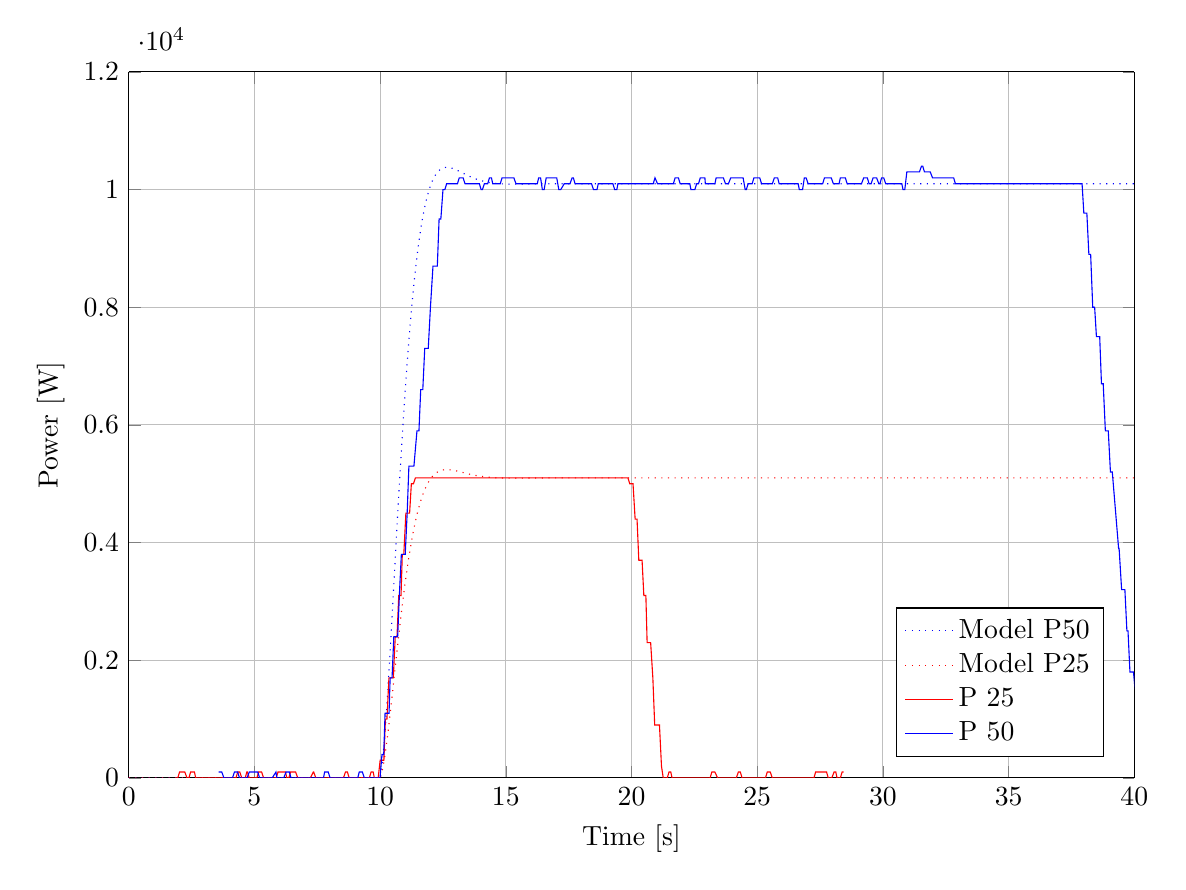
\begin{tikzpicture}

\begin{axis}[%
width=5.028in,
height=3.53in,
at={(0.883in,0.481in)},
scale only axis,
separate axis lines,
every outer x axis line/.append style={black},
every x tick label/.append style={font=\color{black}},
xmin=0,
xmax=40,
xmajorgrids,
xlabel={Time [s]},
every outer y axis line/.append style={black},
every y tick label/.append style={font=\color{black}},
ymin=0,
ymax=12000,
ylabel={Power [W]},
ymajorgrids,
axis background/.style={fill=white},
legend style={at={(0.97,0.03)},anchor=south east,legend cell align=left,align=left,draw=black},
]
\addplot [color=blue,dotted]
 table[row sep=crcr]{%
0	0\\
0.0695737359771018	0\\
0.139147471954204	0\\
0.208721207931306	0\\
0.278294943908407	0\\
0.347868679885509	0\\
0.417442415862611	0\\
0.487016151839713	0\\
0.556589887816815	0\\
0.626163623793917	0\\
0.695737359771018	0\\
0.76531109574812	0\\
0.834884831725222	0\\
0.904458567702324	0\\
0.974032303679426	0\\
1.04360603965653	0\\
1.11317977563363	0\\
1.18275351161073	0\\
1.25232724758783	0\\
1.32190098356493	0\\
1.39147471954204	0\\
1.46104845551914	0\\
1.53062219149624	0\\
1.60019592747334	0\\
1.66976966345044	0\\
1.73934339942755	0\\
1.80891713540465	0\\
1.87849087138175	0\\
1.94806460735885	0\\
2.01763834333595	0\\
2.08721207931306	0\\
2.15678581529016	0\\
2.22635955126726	0\\
2.29593328724436	0\\
2.36550702322146	0\\
2.43508075919856	0\\
2.50465449517567	0\\
2.57422823115277	0\\
2.64380196712987	0\\
2.71337570310697	0\\
2.78294943908407	0\\
2.85252317506118	0\\
2.92209691103828	0\\
2.99167064701538	0\\
3.06124438299248	0\\
3.13081811896958	0\\
3.20039185494668	0\\
3.26996559092379	0\\
3.33953932690089	0\\
3.40911306287799	0\\
3.47868679885509	0\\
3.54826053483219	0\\
3.6178342708093	0\\
3.6874080067864	0\\
3.7569817427635	0\\
3.8265554787406	0\\
3.8961292147177	0\\
3.9657029506948	0\\
4.03527668667191	0\\
4.10485042264901	0\\
4.17442415862611	0\\
4.24399789460321	0\\
4.31357163058031	0\\
4.38314536655742	0\\
4.45271910253452	0\\
4.52229283851162	0\\
4.59186657448872	0\\
4.66144031046582	0\\
4.73101404644293	0\\
4.80058778242003	0\\
4.87016151839713	0\\
4.93973525437423	0\\
5.00930899035133	0\\
5.07888272632843	0\\
5.14845646230554	0\\
5.21803019828264	0\\
5.28760393425974	0\\
5.35717767023684	0\\
5.42675140621394	0\\
5.49632514219105	0\\
5.56589887816815	0\\
5.63547261414525	0\\
5.70504635012235	0\\
5.77462008609945	0\\
5.84419382207656	0\\
5.91376755805366	0\\
5.98334129403076	0\\
6.05291503000786	0\\
6.12248876598496	0\\
6.19206250196206	0\\
6.26163623793917	0\\
6.33120997391627	0\\
6.40078370989337	0\\
6.47035744587047	0\\
6.53993118184757	0\\
6.60950491782468	0\\
6.67907865380178	0\\
6.74865238977888	0\\
6.81822612575598	0\\
6.88779986173308	0\\
6.95737359771018	0\\
7.02694733368729	0\\
7.09652106966439	0\\
7.16609480564149	0\\
7.23566854161859	0\\
7.30524227759569	0\\
7.3748160135728	0\\
7.4443897495499	0\\
7.513963485527	0\\
7.5835372215041	0\\
7.6531109574812	0\\
7.7226846934583	0\\
7.79225842943541	0\\
7.86183216541251	0\\
7.93140590138961	0\\
8.00097963736671	0\\
8.07055337334381	0\\
8.14012710932091	0\\
8.20970084529802	0\\
8.27927458127512	0\\
8.34884831725222	0\\
8.41842205322932	0\\
8.48799578920642	0\\
8.55756952518353	0\\
8.62714326116063	0\\
8.69671699713773	0\\
8.76629073311483	0\\
8.83586446909193	0\\
8.90543820506904	0\\
8.97501194104614	0\\
9.04458567702324	0\\
9.11415941300034	0\\
9.18373314897744	0\\
9.25330688495455	0\\
9.32288062093165	0\\
9.39245435690875	0\\
9.46202809288585	0\\
9.53160182886295	0\\
9.60117556484005	0\\
9.67074930081716	0\\
9.74032303679426	0\\
9.80989677277136	0\\
9.87947050874846	0\\
9.94904424472556	0\\
10.0186179807027	39.1656812783828\\
10.0881917166798	258.174939653554\\
10.1577654526569	574.578087991758\\
10.227339188634	967.674313065982\\
10.2969129246111	1419.199360645\\
10.3664866605882	1913.16473627758\\
10.4360603965653	2435.69291773277\\
10.5056341325424	2974.85149772722\\
10.5752078685195	3520.48869914128\\
10.6447816044966	4064.07227533862\\
10.7143553404737	4598.53342343789\\
10.7839290764508	5118.11699614652\\
10.8535028124279	5618.23899557068\\
10.923076548405	6095.35206764553\\
10.9926502843821	6546.81948580235\\
11.0622240203592	6970.79791449571\\
11.1317977563363	7366.12907456614\\
11.2013714923134	7732.24029047516\\
11.2709452282905	8069.05378166201\\
11.3405189642676	8376.90446417959\\
11.4100927002447	8656.46595203029\\
11.4796664362218	8908.68438803188\\
11.5492401721989	9134.71968952775\\
11.618813908176	9335.89376288467\\
11.6883876441531	9513.64522071241\\
11.7579613801302	9669.49012545367\\
11.8275351161073	9804.98828093474\\
11.8971088520844	9921.71459828085\\
11.9666825880615	10021.2350730634\\
12.0362563240386	10105.0869255666\\
12.1058300600157	10174.7624746658\\
12.1754037959928	10231.6963371441\\
12.2449775319699	10277.2555675845\\
12.314551267947	10312.7323786154\\
12.3841250039241	10339.3391066931\\
12.4536987399012	10358.2051143069\\
12.5232724758783	10370.3753450817\\
12.5928462118554	10376.8102734106\\
12.6624199478325	10378.3870146918\\
12.7319936838096	10375.901385773\\
12.8015674197867	10370.070727639\\
12.8711411557638	10361.5373236052\\
12.9407148917409	10350.8722662087\\
13.010288627718	10338.5796445662\\
13.0798623636951	10325.1009411711\\
13.1494360996722	10310.8195429229\\
13.2190098356494	10296.0652856424\\
13.2885835716265	10281.118964454\\
13.3581573076036	10266.2167542563\\
13.4277310435807	10251.5544951145\\
13.4973047795578	10237.2918068481\\
13.5668785155349	10223.556005428\\
13.636452251512	10210.4458011068\\
13.7060259874891	10198.0347645626\\
13.7755997234662	10186.3745528071\\
13.8451734594433	10175.4978912734\\
13.9147471954204	10165.4213124299\\
13.9843209313975	10156.1476545264\\
14.0538946673746	10147.6683267447\\
14.1234684033517	10139.965349158\\
14.1930421393288	10133.013177559\\
14.2626158753059	10126.7803244607\\
14.332189611283	10121.2307884499\\
14.4017633472601	10116.3253046401\\
14.4713370832372	10112.0224292662\\
14.5409108192143	10108.2794715294\\
14.6104845551914	10105.0532856819\\
14.6800582911685	10102.300936059\\
14.7496320271456	10099.9802473637\\
14.8192057631227	10098.0502520023\\
14.8887794990998	10096.4715456888\\
14.9583532350769	10095.2065619014\\
15.027926971054	10094.2197750985\\
15.0975007070311	10093.4778419085\\
15.1670744430082	10092.9496888018\\
15.2366481789853	10092.6065540542\\
15.3062219149624	10092.421991117\\
15.3757956509395	10092.3718398432\\
15.4453693869166	10092.4341713681\\
15.5149431228937	10092.5892118285\\
15.5845168588708	10092.8192495233\\
15.6540905948479	10093.1085295637\\
15.723664330825	10093.4431395585\\
15.7932380668021	10093.8108893994\\
15.8628118027792	10094.2011877797\\
15.9323855387563	10094.6049176795\\
16.0019592747334	10095.0143126906\\
16.0715330107105	10095.422835726\\
16.1411067466876	10095.8250613668\\
16.2106804826647	10096.2165628406\\
16.2802542186418	10096.5938043924\\
16.3498279546189	10096.9540396099\\
16.419401690596	10097.2952160875\\
16.4889754265731	10097.6158866635\\
16.5585491625502	10097.9151273346\\
16.6281228985273	10098.1924618452\\
16.6976966345044	10098.4477928557\\
16.7672703704815	10098.681339523\\
16.8368441064586	10098.8935812648\\
16.9064178424357	10099.0852074356\\
16.9759915784128	10099.2570726047\\
17.04556531439	10099.4101571056\\
17.1151390503671	10099.5455325059\\
17.1847127863442	10099.6643316431\\
17.2542865223213	10099.7677228648\\
17.3238602582984	10099.8568881193\\
17.3934339942755	10099.9330045454\\
17.4630077302526	10099.9972292266\\
17.5325814662297	10100.050686782\\
17.6021552022068	10100.0944594892\\
17.6717289381839	10100.1295796456\\
17.741302674161	10100.1570238966\\
17.8108764101381	10100.1777092771\\
17.8804501461152	10100.1924907325\\
17.9500238820923	10100.2021599028\\
18.0195976180694	10100.2074449753\\
18.0891713540465	10100.2090114275\\
18.1587450900236	10100.2074635002\\
18.2283188260007	10100.2033462579\\
18.2978925619778	10100.1971481105\\
18.3674662979549	10100.1893036821\\
18.437040033932	10100.1801969323\\
18.5066137699091	10100.1701644422\\
18.5761875058862	10100.1594987947\\
18.6457612418633	10100.1484519856\\
18.7153349778404	10100.1372388149\\
18.7849087138175	10100.1260402145\\
18.8544824497946	10100.1150064783\\
18.9240561857717	10100.1042603666\\
18.9936299217488	10100.0939000639\\
19.0632036577259	10100.0840019742\\
19.132777393703	10100.0746233431\\
19.2023511296801	10100.0658047002\\
19.2719248656572	10100.0575721186\\
19.3414986016343	10100.0499392912\\
19.4110723376114	10100.0429094267\\
19.4806460735885	10100.03647697\\
19.5502198095656	10100.030629152\\
19.6197935455427	10100.0253473775\\
19.6893672815198	10100.0206084591\\
19.7589410174969	10100.016385706\\
19.828514753474	10100.0126498775\\
19.8980884894511	10100.0093700106\\
19.9676622254282	10100.0065141323\\
20.0372359614053	10100.0040498657\\
20.1068096973824	10100.0019449391\\
20.1763834333595	10100.0001676092\\
20.2459571693366	10099.9986870044\\
20.3155309053137	10099.9974733998\\
20.3851046412908	10099.9964984295\\
20.4546783772679	10099.9957352447\\
20.524252113245	10099.9951586251\\
20.5938258492221	10099.9947450485\\
20.6633995851992	10099.9944727262\\
20.7329733211763	10099.9943216086\\
20.8025470571535	10099.9942733658\\
20.8721207931306	10099.9943113485\\
20.9416945291077	10099.9944205325\\
21.0112682650848	10099.9945874498\\
21.0808420010619	10099.9948001109\\
21.150415737039	10099.9950479195\\
21.2199894730161	10099.9953215824\\
21.2895632089932	10099.9956130173\\
21.3591369449703	10099.9959152593\\
21.4287106809474	10099.9962223677\\
21.4982844169245	10099.996529335\\
21.5678581529016	10099.996831998\\
21.6374318888787	10099.9971269526\\
21.7070056248558	10099.9974114725\\
21.7765793608329	10099.9976834325\\
21.84615309681	10099.9979412362\\
21.9157268327871	10099.9981837488\\
21.9853005687642	10099.9984102351\\
22.0548743047413	10099.998620302\\
22.1244480407184	10099.9988138467\\
22.1940217766955	10099.9989910089\\
22.2635955126726	10099.9991521283\\
22.3331692486497	10099.9992977062\\
22.4027429846268	10099.9994283717\\
22.4723167206039	10099.9995448514\\
22.541890456581	10099.999647943\\
22.6114641925581	10099.9997384928\\
22.6810379285352	10099.9998173758\\
22.7506116645123	10099.9998854787\\
22.8201854004894	10099.9999436862\\
22.8897591364665	10099.9999928693\\
22.9593328724436	10100.0000338752\\
23.0289066084207	10100.0000675204\\
23.0984803443978	10100.0000945843\\
23.1680540803749	10100.000115805\\
23.237627816352	10100.000131876\\
23.3072015523291	10100.0001434446\\
23.3767752883062	10100.0001511104\\
23.4463490242833	10100.0001554254\\
23.5159227602604	10100.0001568946\\
23.5854964962375	10100.0001559765\\
23.6550702322146	10100.0001530855\\
23.7246439681917	10100.0001485928\\
23.7942177041688	10100.0001428292\\
23.8637914401459	10100.0001360871\\
23.933365176123	10100.000128623\\
24.0029389121001	10100.0001206604\\
24.0725126480772	10100.0001123915\\
24.1420863840543	10100.0001039808\\
24.2116601200314	10100.0000955668\\
24.2812338560085	10100.0000872649\\
24.3508075919856	10100.0000791694\\
24.4203813279627	10100.000071356\\
24.4899550639398	10100.0000638838\\
24.559528799917	10100.0000567974\\
24.6291025358941	10100.0000501284\\
24.6986762718712	10100.0000438977\\
24.7682500078483	10100.0000381165\\
24.8378237438254	10100.000032788\\
24.9073974798025	10100.0000279087\\
24.9769712157796	10100.0000234696\\
25.0465449517567	10100.0000194572\\
25.1161186877338	10100.0000158545\\
25.1856924237109	10100.0000126416\\
25.255266159688	10100.0000097968\\
25.3248398956651	10100.000007297\\
25.3944136316422	10100.0000051182\\
25.4639873676193	10100.0000032362\\
25.5335611035964	10100.0000016266\\
25.6031348395735	10100.0000002657\\
25.6727085755506	10099.99999913\\
25.7422823115277	10099.9999981973\\
25.8118560475048	10099.9999974461\\
25.8814297834819	10099.9999968562\\
25.951003519459	10099.9999964083\\
26.0205772554361	10099.9999960848\\
26.0901509914132	10099.9999958691\\
26.1597247273903	10099.9999957461\\
26.2292984633674	10099.9999957017\\
26.2988721993445	10099.9999957235\\
26.3684459353216	10099.9999957999\\
26.4380196712987	10099.9999959208\\
26.5075934072758	10099.9999960769\\
26.5771671432529	10099.9999962603\\
26.64674087923	10099.9999964639\\
26.7163146152071	10099.9999966814\\
26.7858883511842	10099.9999969076\\
26.8554620871613	10099.999997138\\
26.9250358231384	10099.9999973686\\
26.9946095591155	10099.9999975963\\
27.0641832950926	10099.9999978185\\
27.1337570310697	10099.999998033\\
27.2033307670468	10099.9999982383\\
27.2729045030239	10099.9999984331\\
27.342478239001	10099.9999986165\\
27.4120519749781	10099.9999987879\\
27.4816257109552	10099.999998947\\
27.5511994469323	10099.9999990937\\
27.6207731829094	10099.9999992281\\
27.6903469188865	10099.9999993504\\
27.7599206548636	10099.999999461\\
27.8294943908407	10099.9999995603\\
27.8990681268178	10099.9999996489\\
27.9686418627949	10099.9999997274\\
28.038215598772	10099.9999997964\\
28.1077893347491	10099.9999998566\\
28.1773630707262	10099.9999999086\\
28.2469368067033	10099.9999999531\\
28.3165105426805	10099.9999999908\\
28.3860842786576	10100.0000000222\\
28.4556580146347	10100.0000000481\\
28.5252317506118	10100.0000000689\\
28.5948054865889	10100.0000000853\\
28.664379222566	10100.0000000978\\
28.7339529585431	10100.0000001069\\
28.8035266945202	10100.0000001129\\
28.8731004304973	10100.0000001164\\
28.9426741664744	10100.0000001178\\
29.0122479024515	10100.0000001173\\
29.0818216384286	10100.0000001152\\
29.1513953744057	10100.000000112\\
29.2209691103828	10100.0000001078\\
29.2905428463599	10100.0000001028\\
29.360116582337	10100.0000000972\\
29.4296903183141	10100.0000000913\\
29.4992640542912	10100.0000000851\\
29.5688377902683	10100.0000000788\\
29.6384115262454	10100.0000000725\\
29.7079852622225	10100.0000000662\\
29.7775589981996	10100.0000000601\\
29.8471327341767	10100.0000000542\\
29.9167064701538	10100.0000000486\\
29.9862802061309	10100.0000000432\\
30.055853942108	10100.0000000382\\
30.1254276780851	10100.0000000335\\
30.1950014140622	10100.0000000291\\
30.2645751500393	10100.0000000251\\
30.3341488860164	10100.0000000214\\
30.4037226219935	10100.000000018\\
30.4732963579706	10100.0000000149\\
30.5428700939477	10100.0000000122\\
30.6124438299248	10100.0000000098\\
30.6820175659019	10100.0000000076\\
30.751591301879	10100.0000000057\\
30.8211650378561	10100.000000004\\
30.8907387738332	10100.0000000026\\
30.9603125098103	10100.0000000014\\
31.0298862457874	10100.0000000003\\
31.0994599817645	10099.9999999995\\
31.1690337177416	10099.9999999987\\
31.2386074537187	10099.9999999982\\
31.3081811896958	10099.9999999977\\
31.3777549256729	10099.9999999974\\
31.44732866165	10099.9999999971\\
31.5169023976271	10099.9999999969\\
31.5864761336042	10099.9999999968\\
31.6560498695813	10099.9999999968\\
31.7256236055584	10099.9999999968\\
31.7951973415355	10099.9999999969\\
31.8647710775126	10099.9999999969\\
31.9343448134897	10099.9999999971\\
32.0039185494668	10099.9999999972\\
32.0734922854439	10099.9999999973\\
32.143066021421	10099.9999999975\\
32.2126397573982	10099.9999999977\\
32.2822134933753	10099.9999999978\\
32.3517872293524	10099.999999998\\
32.4213609653295	10099.9999999982\\
32.4909347013066	10099.9999999984\\
32.5605084372837	10099.9999999985\\
32.6300821732608	10099.9999999987\\
32.6996559092379	10099.9999999988\\
32.769229645215	10099.999999999\\
32.8388033811921	10099.9999999991\\
32.9083771171692	10099.9999999992\\
32.9779508531463	10099.9999999993\\
33.0475245891234	10099.9999999994\\
33.1170983251005	10099.9999999995\\
33.1866720610776	10099.9999999996\\
33.2562457970547	10099.9999999997\\
33.3258195330318	10099.9999999997\\
33.3953932690089	10099.9999999998\\
33.464967004986	10099.9999999999\\
33.5345407409631	10099.9999999999\\
33.6041144769402	10099.9999999999\\
33.6736882129173	10100\\
33.7432619488944	10100\\
33.8128356848715	10100\\
33.8824094208486	10100.0000000001\\
33.9519831568257	10100.0000000001\\
34.0215568928028	10100.0000000001\\
34.0911306287799	10100.0000000001\\
34.160704364757	10100.0000000001\\
34.2302781007341	10100.0000000001\\
34.2998518367112	10100.0000000001\\
34.3694255726883	10100.0000000001\\
34.4389993086654	10100.0000000001\\
34.5085730446425	10100.0000000001\\
34.5781467806196	10100.0000000001\\
34.6477205165967	10100.0000000001\\
34.7172942525738	10100.0000000001\\
34.7868679885509	10100.0000000001\\
34.856441724528	10100.0000000001\\
34.9260154605051	10100.0000000001\\
34.9955891964822	10100.0000000001\\
35.0651629324593	10100.0000000001\\
35.1347366684364	10100.0000000001\\
35.2043104044135	10100.0000000001\\
35.2738841403906	10100.0000000001\\
35.3434578763677	10100\\
35.4130316123448	10100\\
35.4826053483219	10100\\
35.552179084299	10100\\
35.6217528202761	10100\\
35.6913265562532	10100\\
35.7609002922303	10100\\
35.8304740282074	10100\\
35.9000477641845	10100\\
35.9696215001617	10100\\
36.0391952361388	10100\\
36.1087689721159	10100\\
36.178342708093	10100\\
36.2479164440701	10100\\
36.3174901800472	10100\\
36.3870639160243	10100\\
36.4566376520014	10100\\
36.5262113879785	10100\\
36.5957851239556	10100\\
36.6653588599327	10100\\
36.7349325959098	10100\\
36.8045063318869	10100\\
36.874080067864	10100\\
36.9436538038411	10100\\
37.0132275398182	10100\\
37.0828012757953	10100\\
37.1523750117724	10100\\
37.2219487477495	10100\\
37.2915224837266	10100\\
37.3610962197037	10100\\
37.4306699556808	10100\\
37.5002436916579	10100\\
37.569817427635	10100\\
37.6393911636121	10100\\
37.7089648995892	10100\\
37.7785386355663	10100\\
37.8481123715434	10100\\
37.9176861075205	10100\\
37.9872598434976	10100\\
38.0568335794747	10100\\
38.1264073154518	10100\\
38.1959810514289	10100\\
38.265554787406	10100\\
38.3351285233831	10100\\
38.4047022593602	10100\\
38.4742759953373	10100\\
38.5438497313144	10100\\
38.6134234672915	10100\\
38.6829972032686	10100\\
38.7525709392457	10100\\
38.8221446752228	10100\\
38.8917184111999	10100\\
38.961292147177	10100\\
39.0308658831541	10100\\
39.1004396191312	10100\\
39.1700133551083	10100\\
39.2395870910854	10100\\
39.3091608270625	10100\\
39.3787345630396	10100\\
39.4483082990167	10100\\
39.5178820349938	10100\\
39.5874557709709	10100\\
39.657029506948	10100\\
39.7266032429252	10100\\
39.7961769789023	10100\\
39.8657507148794	10100\\
39.9353244508565	10100\\
40.0048981868336	10100\\
};
\addlegendentry{Model P50};

\addplot [color=red,dotted]
 table[row sep=crcr]{%
0	0\\
0.0695737359771018	0\\
0.139147471954204	0\\
0.208721207931306	0\\
0.278294943908407	0\\
0.347868679885509	0\\
0.417442415862611	0\\
0.487016151839713	0\\
0.556589887816815	0\\
0.626163623793917	0\\
0.695737359771018	0\\
0.76531109574812	0\\
0.834884831725222	0\\
0.904458567702324	0\\
0.974032303679426	0\\
1.04360603965653	0\\
1.11317977563363	0\\
1.18275351161073	0\\
1.25232724758783	0\\
1.32190098356493	0\\
1.39147471954204	0\\
1.46104845551914	0\\
1.53062219149624	0\\
1.60019592747334	0\\
1.66976966345044	0\\
1.73934339942755	0\\
1.80891713540465	0\\
1.87849087138175	0\\
1.94806460735885	0\\
2.01763834333595	0\\
2.08721207931306	0\\
2.15678581529016	0\\
2.22635955126726	0\\
2.29593328724436	0\\
2.36550702322146	0\\
2.43508075919856	0\\
2.50465449517567	0\\
2.57422823115277	0\\
2.64380196712987	0\\
2.71337570310697	0\\
2.78294943908407	0\\
2.85252317506118	0\\
2.92209691103828	0\\
2.99167064701538	0\\
3.06124438299248	0\\
3.13081811896958	0\\
3.20039185494668	0\\
3.26996559092379	0\\
3.33953932690089	0\\
3.40911306287799	0\\
3.47868679885509	0\\
3.54826053483219	0\\
3.6178342708093	0\\
3.6874080067864	0\\
3.7569817427635	0\\
3.8265554787406	0\\
3.8961292147177	0\\
3.9657029506948	0\\
4.03527668667191	0\\
4.10485042264901	0\\
4.17442415862611	0\\
4.24399789460321	0\\
4.31357163058031	0\\
4.38314536655742	0\\
4.45271910253452	0\\
4.52229283851162	0\\
4.59186657448872	0\\
4.66144031046582	0\\
4.73101404644293	0\\
4.80058778242003	0\\
4.87016151839713	0\\
4.93973525437423	0\\
5.00930899035133	0\\
5.07888272632843	0\\
5.14845646230554	0\\
5.21803019828264	0\\
5.28760393425974	0\\
5.35717767023684	0\\
5.42675140621394	0\\
5.49632514219105	0\\
5.56589887816815	0\\
5.63547261414525	0\\
5.70504635012235	0\\
5.77462008609945	0\\
5.84419382207656	0\\
5.91376755805366	0\\
5.98334129403076	0\\
6.05291503000786	0\\
6.12248876598496	0\\
6.19206250196206	0\\
6.26163623793917	0\\
6.33120997391627	0\\
6.40078370989337	0\\
6.47035744587047	0\\
6.53993118184757	0\\
6.60950491782468	0\\
6.67907865380178	0\\
6.74865238977888	0\\
6.81822612575598	0\\
6.88779986173308	0\\
6.95737359771018	0\\
7.02694733368729	0\\
7.09652106966439	0\\
7.16609480564149	0\\
7.23566854161859	0\\
7.30524227759569	0\\
7.3748160135728	0\\
7.4443897495499	0\\
7.513963485527	0\\
7.5835372215041	0\\
7.6531109574812	0\\
7.7226846934583	0\\
7.79225842943541	0\\
7.86183216541251	0\\
7.93140590138961	0\\
8.00097963736671	0\\
8.07055337334381	0\\
8.14012710932091	0\\
8.20970084529802	0\\
8.27927458127512	0\\
8.34884831725222	0\\
8.41842205322932	0\\
8.48799578920642	0\\
8.55756952518353	0\\
8.62714326116063	0\\
8.69671699713773	0\\
8.76629073311483	0\\
8.83586446909193	0\\
8.90543820506904	0\\
8.97501194104614	0\\
9.04458567702324	0\\
9.11415941300034	0\\
9.18373314897744	0\\
9.25330688495455	0\\
9.32288062093165	0\\
9.39245435690875	0\\
9.46202809288585	0\\
9.53160182886295	0\\
9.60117556484005	0\\
9.67074930081716	0\\
9.74032303679426	0\\
9.80989677277136	0\\
9.87947050874846	0\\
9.94904424472556	0\\
10.0186179807027	19.7767301504705\\
10.0881917166798	130.365563587438\\
10.1577654526569	290.133489976036\\
10.227339188634	488.627623429357\\
10.2969129246111	716.625419731636\\
10.3664866605882	966.053480694619\\
10.4360603965653	1229.90434459773\\
10.5056341325424	1502.15273647612\\
10.5752078685195	1777.67251144757\\
10.6447816044966	2052.1553073492\\
10.7143553404737	2322.03172866666\\
10.7839290764508	2584.39571092547\\
10.8535028124279	2836.93256211985\\
10.923076548405	3077.85104405864\\
10.9926502843821	3305.81974035564\\
11.0622240203592	3519.90785781466\\
11.1317977563363	3719.53052280073\\
11.2013714923134	3904.39856251716\\
11.2709452282905	4074.47270163131\\
11.3405189642676	4229.92205616989\\
11.4100927002447	4371.08676785688\\
11.4796664362218	4498.4445919765\\
11.5492401721989	4612.5812293655\\
11.618813908176	4714.1641772982\\
11.6883876441531	4803.91986392409\\
11.7579613801302	4882.61382572413\\
11.8275351161073	4951.03368641259\\
11.8971088520844	5009.97469814182\\
11.9666825880615	5060.22761115083\\
12.0362563240386	5102.56864558314\\
12.1058300600157	5137.75134859363\\
12.1754037959928	5166.50013063712\\
12.2449775319699	5189.50528660209\\
12.314551267947	5207.4193198949\\
12.3841250039241	5220.85440040938\\
12.4536987399012	5230.38080029356\\
12.5232724758783	5236.52616434821\\
12.5928462118554	5239.77548459349\\
12.6624199478325	5240.57166088397\\
12.7319936838096	5239.31654133091\\
12.8015674197867	5236.37234761967\\
12.8711411557638	5232.06340102835\\
12.9407148917409	5226.67807501626\\
13.010288627718	5220.47090963245\\
13.0798623636951	5213.66483168048\\
13.1494360996722	5206.45343256502\\
13.2190098356494	5199.00326304714\\
13.2885835716265	5191.45611076389\\
13.3581573076036	5183.93123234722\\
13.4277310435807	5176.52751733502\\
13.4973047795578	5169.32556583419\\
13.5668785155349	5162.3896661072\\
13.636452251512	5155.76966194501\\
13.7060259874891	5149.50270289797\\
13.7755997234662	5143.61487319962\\
13.8451734594433	5138.12269757368\\
13.9147471954204	5133.03452409828\\
13.9843209313975	5128.35178594899\\
14.0538946673746	5124.07014518793\\
14.1234684033517	5120.18052284214\\
14.1930421393288	5116.67002035156\\
14.2626158753059	5113.52273809401\\
14.332189611283	5110.72049713804\\
14.4017633472601	5108.24347065985\\
14.4713370832372	5106.07073160966\\
14.5409108192143	5104.18072324752\\
14.6104845551914	5102.55165910669\\
14.6800582911685	5101.16185880205\\
14.7496320271456	5099.99002589653\\
14.8192057631227	5099.01547378335\\
14.8887794990998	5098.21830524882\\
14.9583532350769	5097.57955105914\\
15.027926971054	5097.0812725745\\
15.0975007070311	5096.70663304289\\
15.1670744430082	5096.43994187022\\
15.2366481789853	5096.26667580952\\
15.3062219149624	5096.17348066303\\
15.3757956509395	5096.14815675253\\
15.4453693869166	5096.17963108684\\
15.5149431228937	5096.25791884412\\
15.5845168588708	5096.37407649196\\
15.6540905948479	5096.52014859156\\
15.723664330825	5096.6891100741\\
15.7932380668021	5096.87480553833\\
15.8628118027792	5097.07188689865\\
15.9323855387563	5097.27575051141\\
16.0019592747334	5097.48247472497\\
16.0715330107105	5097.68875863392\\
16.1411067466876	5097.89186267037\\
16.2106804826647	5098.08955153336\\
16.2802542186418	5098.28003984169\\
16.3498279546189	5098.46194079312\\
16.419401690596	5098.6342180244\\
16.4889754265731	5098.79614079049\\
16.5585491625502	5098.94724251551\\
16.6281228985273	5099.08728271393\\
16.6976966345044	5099.21621223409\\
16.7672703704815	5099.33414173934\\
16.8368441064586	5099.44131331194\\
16.9064178424357	5099.53807504173\\
16.9759915784128	5099.62485844397\\
17.04556531439	5099.70215853847\\
17.1151390503671	5099.77051641387\\
17.1847127863442	5099.83050409699\\
17.2542865223213	5099.88271154559\\
17.3238602582984	5099.92773558497\\
17.3934339942755	5099.96617061205\\
17.4630077302526	5099.99860089659\\
17.5325814662297	5100.02559431565\\
17.6021552022068	5100.04769736584\\
17.6717289381839	5100.06543130619\\
17.741302674161	5100.0792892943\\
17.8108764101381	5100.08973438746\\
17.8804501461152	5100.09719829069\\
17.9500238820923	5100.10208074301\\
18.0195976180694	5100.10474944299\\
18.0891713540465	5100.1055404238\\
18.1587450900236	5100.10475879711\\
18.2283188260007	5100.10267979362\\
18.2978925619778	5100.099550036\\
18.3674662979549	5100.09558898801\\
18.437040033932	5100.09099053018\\
18.5066137699091	5100.08592461933\\
18.5761875058862	5100.08053899534\\
18.6457612418633	5100.07496090362\\
18.7153349778404	5100.06929880752\\
18.7849087138175	5100.0636440687\\
18.8544824497946	5100.05807257814\\
18.9240561857717	5100.05264632372\\
18.9936299217488	5100.04741488374\\
19.0632036577259	5100.04241683843\\
19.132777393703	5100.03768109402\\
19.2023511296801	5100.03322811595\\
19.2719248656572	5100.0290710698\\
19.3414986016343	5100.02521686981\\
19.4110723376114	5100.02166713627\\
19.4806460735885	5100.01841906407\\
19.5502198095656	5100.01546620545\\
19.6197935455427	5100.01279917079\\
19.6893672815198	5100.01040625161\\
19.7589410174969	5100.00827397035\\
19.828514753474	5100.00638756188\\
19.8980884894511	5100.00473139147\\
19.9676622254282	5100.00328931433\\
20.0372359614053	5100.00204498167\\
20.1068096973824	5100.00098209798\\
20.1763834333595	5100.00008463435\\
20.2459571693366	5099.99933700224\\
20.3155309053137	5099.99872419199\\
20.3851046412908	5099.99823188023\\
20.4546783772679	5099.9978465097\\
20.524252113245	5099.99755534533\\
20.5938258492221	5099.99734650963\\
20.6633995851992	5099.99720900037\\
20.7329733211763	5099.99713269345\\
20.8025470571535	5099.99710833322\\
20.8721207931306	5099.99712751262\\
20.9416945291077	5099.99718264511\\
21.0112682650848	5099.99726693009\\
21.0808420010619	5099.99737431344\\
21.150415737039	5099.9974994445\\
21.2199894730161	5099.99763763072\\
21.2895632089932	5099.99778479093\\
21.3591369449703	5099.99793740817\\
21.4287106809474	5099.99809248271\\
21.4982844169245	5099.998247486\\
21.5678581529016	5099.99840031582\\
21.6374318888787	5099.99854925328\\
21.7070056248558	5099.99869292176\\
21.7765793608329	5099.99883024811\\
21.84615309681	5099.99896042621\\
21.9157268327871	5099.99908288307\\
21.9853005687642	5099.99919724742\\
22.0548743047413	5099.99930332082\\
22.1244480407184	5099.9994010513\\
22.1940217766955	5099.99949050943\\
22.2635955126726	5099.99957186674\\
22.3331692486497	5099.9996453764\\
22.4027429846268	5099.99971135602\\
22.4723167206039	5099.99977017248\\
22.541890456581	5099.99982222865\\
22.6114641925581	5099.99986795183\\
22.6810379285352	5099.99990778381\\
22.7506116645123	5099.9999421724\\
22.8201854004894	5099.99997156434\\
22.8897591364665	5099.99999639934\\
22.9593328724436	5100.00001710531\\
23.0289066084207	5100.00003409446\\
23.0984803443978	5100.0000477604\\
23.1680540803749	5100.00005847579\\
23.237627816352	5100.00006659087\\
23.3072015523291	5100.00007243243\\
23.3767752883062	5100.00007630327\\
23.4463490242833	5100.00007848214\\
23.5159227602604	5100.00007922398\\
23.5854964962375	5100.00007876043\\
23.6550702322146	5100.0000773006\\
23.7246439681917	5100.00007503201\\
23.7942177041688	5100.00007212166\\
23.8637914401459	5100.00006871723\\
23.933365176123	5100.00006494827\\
24.0029389121001	5100.00006092751\\
24.0725126480772	5100.00005675216\\
24.1420863840543	5100.00005250517\\
24.2116601200314	5100.00004825653\\
24.2812338560085	5100.00004406446\\
24.3508075919856	5100.00003997662\\
24.4203813279627	5100.00003603124\\
24.4899550639398	5100.00003225816\\
24.559528799917	5100.00002867986\\
24.6291025358941	5100.00002531238\\
24.6986762718712	5100.00002216617\\
24.7682500078483	5100.00001924693\\
24.8378237438254	5100.0000165563\\
24.9073974798025	5100.0000140925\\
24.9769712157796	5100.00001185098\\
25.0465449517567	5100.00000982493\\
25.1161186877338	5100.00000800572\\
25.1856924237109	5100.00000638338\\
25.255266159688	5100.0000049469\\
25.3248398956651	5100.00000368462\\
25.3944136316422	5100.00000258444\\
25.4639873676193	5100.00000163411\\
25.5335611035964	5100.00000082136\\
25.6031348395735	5100.00000013415\\
25.6727085755506	5099.99999956072\\
25.7422823115277	5099.99999908975\\
25.8118560475048	5099.99999871043\\
25.8814297834819	5099.99999841252\\
25.951003519459	5099.99999818638\\
26.0205772554361	5099.99999802302\\
26.0901509914132	5099.99999791411\\
26.1597247273903	5099.99999785197\\
26.2292984633674	5099.99999782959\\
26.2988721993445	5099.99999784057\\
26.3684459353216	5099.99999787916\\
26.4380196712987	5099.99999794019\\
26.5075934072758	5099.99999801905\\
26.5771671432529	5099.99999811166\\
26.64674087923	5099.99999821444\\
26.7163146152071	5099.99999832429\\
26.7858883511842	5099.99999843851\\
26.8554620871613	5099.99999855481\\
26.9250358231384	5099.99999867126\\
26.9946095591155	5099.99999878625\\
27.0641832950926	5099.99999889844\\
27.1337570310697	5099.99999900678\\
27.2033307670468	5099.99999911045\\
27.2729045030239	5099.9999992088\\
27.342478239001	5099.99999930141\\
27.4120519749781	5099.99999938796\\
27.4816257109552	5099.9999994683\\
27.5511994469323	5099.99999954237\\
27.6207731829094	5099.99999961023\\
27.6903469188865	5099.99999967198\\
27.7599206548636	5099.99999972782\\
27.8294943908407	5099.99999977798\\
27.8990681268178	5099.99999982273\\
27.9686418627949	5099.99999986237\\
28.038215598772	5099.99999989721\\
28.1077893347491	5099.9999999276\\
28.1773630707262	5099.99999995386\\
28.2469368067033	5099.99999997633\\
28.3165105426805	5099.99999999535\\
28.3860842786576	5100.00000001123\\
28.4556580146347	5100.00000002428\\
28.5252317506118	5100.00000003481\\
28.5948054865889	5100.00000004309\\
28.664379222566	5100.00000004939\\
28.7339529585431	5100.00000005396\\
28.8035266945202	5100.00000005702\\
28.8731004304973	5100.00000005879\\
28.9426741664744	5100.00000005946\\
29.0122479024515	5100.00000005921\\
29.0818216384286	5100.00000005819\\
29.1513953744057	5100.00000005655\\
29.2209691103828	5100.00000005442\\
29.2905428463599	5100.0000000519\\
29.360116582337	5100.0000000491\\
29.4296903183141	5100.0000000461\\
29.4992640542912	5100.00000004297\\
29.5688377902683	5100.00000003979\\
29.6384115262454	5100.00000003659\\
29.7079852622225	5100.00000003344\\
29.7775589981996	5100.00000003036\\
29.8471327341767	5100.00000002739\\
29.9167064701538	5100.00000002454\\
29.9862802061309	5100.00000002184\\
30.055853942108	5100.00000001929\\
30.1254276780851	5100.00000001691\\
30.1950014140622	5100.0000000147\\
30.2645751500393	5100.00000001266\\
30.3341488860164	5100.00000001079\\
30.4037226219935	5100.00000000909\\
30.4732963579706	5100.00000000755\\
30.5428700939477	5100.00000000617\\
30.6124438299248	5100.00000000493\\
30.6820175659019	5100.00000000384\\
30.751591301879	5100.00000000288\\
30.8211650378561	5100.00000000204\\
30.8907387738332	5100.00000000131\\
30.9603125098103	5100.00000000069\\
31.0298862457874	5100.00000000016\\
31.0994599817645	5099.99999999972\\
31.1690337177416	5099.99999999936\\
31.2386074537187	5099.99999999907\\
31.3081811896958	5099.99999999884\\
31.3777549256729	5099.99999999866\\
31.44732866165	5099.99999999853\\
31.5169023976271	5099.99999999845\\
31.5864761336042	5099.9999999984\\
31.6560498695813	5099.99999999838\\
31.7256236055584	5099.99999999838\\
31.7951973415355	5099.99999999841\\
31.8647710775126	5099.99999999845\\
31.9343448134897	5099.99999999851\\
32.0039185494668	5099.99999999858\\
32.0734922854439	5099.99999999866\\
32.143066021421	5099.99999999874\\
32.2126397573982	5099.99999999882\\
32.2822134933753	5099.99999999891\\
32.3517872293524	5099.999999999\\
32.4213609653295	5099.99999999909\\
32.4909347013066	5099.99999999917\\
32.5605084372837	5099.99999999925\\
32.6300821732608	5099.99999999933\\
32.6996559092379	5099.9999999994\\
32.769229645215	5099.99999999947\\
32.8388033811921	5099.99999999954\\
32.9083771171692	5099.9999999996\\
32.9779508531463	5099.99999999966\\
33.0475245891234	5099.99999999971\\
33.1170983251005	5099.99999999976\\
33.1866720610776	5099.9999999998\\
33.2562457970547	5099.99999999984\\
33.3258195330318	5099.99999999987\\
33.3953932690089	5099.9999999999\\
33.464967004986	5099.99999999993\\
33.5345407409631	5099.99999999995\\
33.6041144769402	5099.99999999997\\
33.6736882129173	5099.99999999999\\
33.7432619488944	5100\\
33.8128356848715	5100.00000000002\\
33.8824094208486	5100.00000000003\\
33.9519831568257	5100.00000000003\\
34.0215568928028	5100.00000000004\\
34.0911306287799	5100.00000000005\\
34.160704364757	5100.00000000005\\
34.2302781007341	5100.00000000005\\
34.2998518367112	5100.00000000005\\
34.3694255726883	5100.00000000005\\
34.4389993086654	5100.00000000005\\
34.5085730446425	5100.00000000005\\
34.5781467806196	5100.00000000005\\
34.6477205165967	5100.00000000005\\
34.7172942525738	5100.00000000005\\
34.7868679885509	5100.00000000005\\
34.856441724528	5100.00000000004\\
34.9260154605051	5100.00000000004\\
34.9955891964822	5100.00000000004\\
35.0651629324593	5100.00000000004\\
35.1347366684364	5100.00000000003\\
35.2043104044135	5100.00000000003\\
35.2738841403906	5100.00000000003\\
35.3434578763677	5100.00000000002\\
35.4130316123448	5100.00000000002\\
35.4826053483219	5100.00000000002\\
35.552179084299	5100.00000000002\\
35.6217528202761	5100.00000000002\\
35.6913265562532	5100.00000000001\\
35.7609002922303	5100.00000000001\\
35.8304740282074	5100.00000000001\\
35.9000477641845	5100.00000000001\\
35.9696215001617	5100.00000000001\\
36.0391952361388	5100.00000000001\\
36.1087689721159	5100.00000000001\\
36.178342708093	5100.00000000001\\
36.2479164440701	5100.00000000001\\
36.3174901800472	5100.00000000001\\
36.3870639160243	5100\\
36.4566376520014	5100\\
36.5262113879785	5100\\
36.5957851239556	5100\\
36.6653588599327	5100\\
36.7349325959098	5100\\
36.8045063318869	5100\\
36.874080067864	5100\\
36.9436538038411	5100\\
37.0132275398182	5100\\
37.0828012757953	5100\\
37.1523750117724	5100\\
37.2219487477495	5100\\
37.2915224837266	5100\\
37.3610962197037	5100\\
37.4306699556808	5100\\
37.5002436916579	5100\\
37.569817427635	5100\\
37.6393911636121	5100\\
37.7089648995892	5100\\
37.7785386355663	5100\\
37.8481123715434	5100\\
37.9176861075205	5100\\
37.9872598434976	5100\\
38.0568335794747	5100\\
38.1264073154518	5100\\
38.1959810514289	5100\\
38.265554787406	5100\\
38.3351285233831	5100\\
38.4047022593602	5100\\
38.4742759953373	5100\\
38.5438497313144	5100\\
38.6134234672915	5100\\
38.6829972032686	5100\\
38.7525709392457	5100\\
38.8221446752228	5100\\
38.8917184111999	5100\\
38.961292147177	5100\\
39.0308658831541	5100\\
39.1004396191312	5100\\
39.1700133551083	5100\\
39.2395870910854	5100\\
39.3091608270625	5100\\
39.3787345630396	5100\\
39.4483082990167	5100\\
39.5178820349938	5100\\
39.5874557709709	5100\\
39.657029506948	5100\\
39.7266032429252	5100\\
39.7961769789023	5100\\
39.8657507148794	5100\\
39.9353244508565	5100\\
40.0048981868336	5100\\
};
\addlegendentry{Model P25};

\addplot [color=red,solid]
 table[row sep=crcr]{%
1.882	0\\
1.952	0\\
2.022	100\\
2.102	100\\
2.162	100\\
2.232	100\\
2.318	0\\
2.393	0\\
2.463	100\\
2.532	100\\
2.616	100\\
2.663	0\\
2.733	0\\
2.816	0\\
2.893	0\\
2.964	0\\
3.033	0\\
3.083	0\\
3.163	0\\
3.233	0\\
3.317	0\\
3.394	0\\
3.464	0\\
3.535	0\\
3.585	0\\
3.665	0\\
3.735	0\\
3.82	0\\
3.865	0\\
3.935	0\\
4.055	0\\
4.075	0\\
4.145	0\\
4.195	0\\
4.266	0\\
4.336	100\\
4.419	100\\
4.495	0\\
4.636	0\\
4.696	100\\
4.722	100\\
4.796	0\\
4.876	0\\
4.956	0\\
5.006	0\\
5.096	0\\
5.166	100\\
5.236	100\\
5.286	100\\
5.367	0\\
5.437	0\\
5.521	0\\
5.597	0\\
5.677	0\\
5.721	0\\
5.797	0\\
5.868	0\\
5.937	100\\
6.019	100\\
6.097	100\\
6.167	100\\
6.238	100\\
6.288	0\\
6.368	0\\
6.438	100\\
6.522	100\\
6.578	100\\
6.639	100\\
6.725	0\\
6.799	0\\
6.869	0\\
6.939	0\\
7.021	0\\
7.07	0\\
7.14	0\\
7.225	0\\
7.34	100\\
7.36	100\\
7.44	0\\
7.49	0\\
7.57	0\\
7.65	0\\
7.7	0\\
7.77	0\\
7.823	0\\
7.9	0\\
7.97	0\\
8.04	0\\
8.123	0\\
8.2	0\\
8.27	0\\
8.324	0\\
8.4	0\\
8.47	0\\
8.54	0\\
8.623	100\\
8.7	100\\
8.77	0\\
8.84	0\\
8.922	0\\
9	0\\
9.07	0\\
9.14	0\\
9.223	0\\
9.27	0\\
9.34	0\\
9.423	0\\
9.5	0\\
9.571	0\\
9.641	100\\
9.724	100\\
9.771	0\\
9.841	0\\
9.923	0\\
10.001	300\\
10.071	300\\
10.151	300\\
10.211	1000\\
10.272	1000\\
10.351	1700\\
10.401	1700\\
10.471	1700\\
10.524	1700\\
10.602	2400\\
10.671	2400\\
10.742	3100\\
10.832	3100\\
10.882	3800\\
10.942	3800\\
11.025	4500\\
11.102	4500\\
11.173	4500\\
11.243	5000\\
11.326	5000\\
11.403	5100\\
11.472	5100\\
11.528	5100\\
11.603	5100\\
11.673	5100\\
11.726	5100\\
11.803	5100\\
11.932	5100\\
11.943	5100\\
12.029	5100\\
12.103	5100\\
12.173	5100\\
12.227	5100\\
12.304	5100\\
12.374	5100\\
12.444	5100\\
12.528	5100\\
12.604	5100\\
12.674	5100\\
12.728	5100\\
12.805	5100\\
12.875	5100\\
12.944	5100\\
13.027	5100\\
13.105	5100\\
13.175	5100\\
13.228	5100\\
13.305	5100\\
13.376	5100\\
13.429	5100\\
13.507	5100\\
13.577	5100\\
13.646	5100\\
13.729	5100\\
13.807	5100\\
13.877	5100\\
13.934	5100\\
14.008	5100\\
14.077	5100\\
14.147	5100\\
14.23	5100\\
14.307	5100\\
14.377	5100\\
14.431	5100\\
14.518	5100\\
14.578	5100\\
14.718	5100\\
14.732	5100\\
14.809	5100\\
14.879	5100\\
14.949	5100\\
15.034	5100\\
15.11	5100\\
15.179	5100\\
15.25	5100\\
15.332	5100\\
15.379	5100\\
15.449	5100\\
15.532	5100\\
15.609	5100\\
15.68	5100\\
15.75	5100\\
15.837	5100\\
15.881	5100\\
15.95	5100\\
16.034	5100\\
16.11	5100\\
16.181	5100\\
16.252	5100\\
16.302	5100\\
16.382	5100\\
16.452	5100\\
16.535	5100\\
16.582	5100\\
16.652	5100\\
16.735	5100\\
16.813	5100\\
16.893	5100\\
16.937	5100\\
17.013	5100\\
17.083	5100\\
17.153	5100\\
17.223	5100\\
17.323	5100\\
17.384	5100\\
17.455	5100\\
17.505	5100\\
17.575	5100\\
17.656	5100\\
17.738	5100\\
17.786	5100\\
17.856	5100\\
17.94	5100\\
18.027	5100\\
18.087	5100\\
18.157	5100\\
18.207	5100\\
18.278	5100\\
18.358	5100\\
18.441	5100\\
18.488	5100\\
18.558	5100\\
18.641	5100\\
18.718	5100\\
18.788	5100\\
18.858	5100\\
18.944	5100\\
18.989	5100\\
19.058	5100\\
19.142	5100\\
19.219	5100\\
19.289	5100\\
19.359	5100\\
19.444	5100\\
19.489	5100\\
19.559	5100\\
19.642	5100\\
19.719	5100\\
19.789	5100\\
19.859	5100\\
19.929	5000\\
19.99	5000\\
20.06	5000\\
20.144	4400\\
20.22	4400\\
20.29	3700\\
20.4	3700\\
20.42	3700\\
20.49	3100\\
20.571	3100\\
20.621	2300\\
20.691	2300\\
20.761	2300\\
20.849	1700\\
20.922	900\\
20.992	900\\
21.062	900\\
21.112	900\\
21.192	200\\
21.262	0\\
21.348	0\\
21.422	0\\
21.492	100\\
21.562	100\\
21.613	0\\
21.683	0\\
21.763	0\\
21.848	0\\
21.923	0\\
21.993	0\\
22.064	0\\
22.114	0\\
22.184	0\\
22.264	0\\
22.35	0\\
22.394	0\\
22.464	0\\
22.547	0\\
22.634	0\\
22.674	0\\
22.748	0\\
22.824	0\\
22.895	0\\
22.965	0\\
23.047	0\\
23.125	0\\
23.195	100\\
23.266	100\\
23.316	100\\
23.425	0\\
23.457	0\\
23.537	0\\
23.597	0\\
23.668	0\\
23.752	0\\
23.828	0\\
23.898	0\\
23.968	0\\
24.05	0\\
24.098	0\\
24.168	0\\
24.25	100\\
24.328	100\\
24.398	0\\
24.468	0\\
24.518	0\\
24.598	0\\
24.669	0\\
24.752	0\\
24.829	0\\
24.898	0\\
24.968	0\\
25.018	0\\
25.099	0\\
25.169	0\\
25.252	0\\
25.329	0\\
25.399	100\\
25.469	100\\
25.519	100\\
25.599	0\\
25.669	0\\
25.752	0\\
25.819	0\\
25.86	0\\
25.94	0\\
26	0\\
26.055	0\\
26.13	0\\
26.2	0\\
26.27	0\\
26.34	0\\
26.421	0\\
26.471	0\\
26.556	0\\
26.632	0\\
26.692	0\\
26.755	0\\
26.822	0\\
26.902	0\\
26.962	0\\
27.054	0\\
27.123	0\\
27.203	0\\
27.257	0\\
27.323	100\\
27.404	100\\
27.458	100\\
27.524	100\\
27.605	100\\
27.675	100\\
27.759	100\\
27.825	0\\
27.905	0\\
27.966	0\\
28.057	100\\
28.126	100\\
28.176	0\\
28.246	0\\
28.307	0\\
28.377	100\\
28.437	100\\
};
\addlegendentry{P 25};
\addplot [color=blue,solid]
 table[row sep=crcr]{%
3.573	100\\
3.634	100\\
3.704	100\\
3.785	0\\
3.874	0\\
3.934	0\\
4.005	0\\
4.055	0\\
4.126	0\\
4.205	100\\
4.289	100\\
4.336	100\\
4.406	0\\
4.489	0\\
4.566	0\\
4.636	0\\
4.706	0\\
4.796	100\\
4.846	100\\
4.906	100\\
4.989	100\\
5.066	100\\
5.136	100\\
5.206	0\\
5.294	0\\
5.337	0\\
5.407	0\\
5.49	0\\
5.567	0\\
5.637	0\\
5.707	0\\
5.857	100\\
5.892	0\\
5.957	0\\
6.007	0\\
6.09	0\\
6.167	0\\
6.257	100\\
6.307	100\\
6.39	100\\
6.457	0\\
6.527	0\\
6.598	0\\
6.678	0\\
6.738	0\\
6.808	0\\
6.891	0\\
6.968	0\\
7.038	0\\
7.093	0\\
7.168	0\\
7.238	0\\
7.308	0\\
7.392	0\\
7.458	0\\
7.548	0\\
7.638	0\\
7.658	0\\
7.748	0\\
7.792	100\\
7.868	100\\
7.938	100\\
8.008	0\\
8.092	0\\
8.168	0\\
8.238	0\\
8.291	0\\
8.369	0\\
8.439	0\\
8.509	0\\
8.591	0\\
8.669	0\\
8.739	0\\
8.792	0\\
8.869	0\\
8.94	0\\
9.01	0\\
9.111	0\\
9.17	100\\
9.211	100\\
9.294	100\\
9.372	0\\
9.452	0\\
9.496	0\\
9.572	0\\
9.653	0\\
9.696	0\\
9.773	0\\
9.843	0\\
9.914	0\\
9.997	0\\
10.074	400\\
10.144	400\\
10.197	1100\\
10.274	1100\\
10.355	1100\\
10.399	1700\\
10.475	1700\\
10.545	2400\\
10.615	2400\\
10.698	2400\\
10.776	3200\\
10.845	3800\\
10.915	3800\\
10.999	3800\\
11.076	4500\\
11.145	5300\\
11.199	5300\\
11.276	5300\\
11.345	5300\\
11.466	5900\\
11.475	5900\\
11.545	5900\\
11.615	6600\\
11.698	6600\\
11.775	7300\\
11.845	7300\\
11.915	7300\\
12.002	8000\\
12.103	8700\\
12.146	8700\\
12.199	8700\\
12.276	8700\\
12.346	9500\\
12.416	9500\\
12.501	10000\\
12.576	10000\\
12.646	10100\\
12.699	10100\\
12.776	10100\\
12.846	10100\\
12.917	10100\\
13	10100\\
13.077	10100\\
13.147	10200\\
13.217	10200\\
13.302	10200\\
13.377	10100\\
13.447	10100\\
13.517	10100\\
13.605	10100\\
13.647	10100\\
13.717	10100\\
13.803	10100\\
13.878	10100\\
13.948	10100\\
14.018	10000\\
14.068	10000\\
14.149	10100\\
14.202	10100\\
14.279	10100\\
14.349	10200\\
14.429	10200\\
14.479	10100\\
14.549	10100\\
14.619	10100\\
14.702	10100\\
14.78	10100\\
14.85	10200\\
14.92	10200\\
15.003	10200\\
15.15	10200\\
15.18	10200\\
15.251	10200\\
15.321	10200\\
15.403	10100\\
15.481	10100\\
15.541	10100\\
15.612	10100\\
15.692	10100\\
15.752	10100\\
15.821	10100\\
15.904	10100\\
15.982	10100\\
16.052	10100\\
16.104	10100\\
16.182	10100\\
16.252	10100\\
16.306	10200\\
16.383	10200\\
16.453	10000\\
16.524	10000\\
16.606	10200\\
16.683	10200\\
16.754	10200\\
16.808	10200\\
16.884	10200\\
16.955	10200\\
17.025	10200\\
17.108	10000\\
17.185	10000\\
17.325	10100\\
17.345	10100\\
17.413	10100\\
17.486	10100\\
17.555	10100\\
17.636	10200\\
17.686	10200\\
17.756	10100\\
17.826	10100\\
17.91	10100\\
17.986	10100\\
18.066	10100\\
18.11	10100\\
18.186	10100\\
18.256	10100\\
18.326	10100\\
18.41	10100\\
18.487	10000\\
18.557	10000\\
18.627	10000\\
18.677	10100\\
18.748	10100\\
18.818	10100\\
18.898	10100\\
18.959	10100\\
19.029	10100\\
19.114	10100\\
19.189	10100\\
19.259	10100\\
19.33	10000\\
19.416	10000\\
19.46	10100\\
19.53	10100\\
19.614	10100\\
19.69	10100\\
19.771	10100\\
19.821	10100\\
19.915	10100\\
19.961	10100\\
20.041	10100\\
20.101	10100\\
20.182	10100\\
20.223	10100\\
20.303	10100\\
20.393	10100\\
20.463	10100\\
20.544	10100\\
20.617	10100\\
20.674	10100\\
20.722	10100\\
20.794	10100\\
20.864	10100\\
20.934	10200\\
21.034	10100\\
21.094	10100\\
21.164	10100\\
21.244	10100\\
21.345	10100\\
21.365	10100\\
21.434	10100\\
21.523	10100\\
21.595	10100\\
21.665	10100\\
21.734	10200\\
21.818	10200\\
21.865	10200\\
21.935	10100\\
22.018	10100\\
22.085	10100\\
22.165	10100\\
22.235	10100\\
22.318	10100\\
22.365	10000\\
22.435	10000\\
22.518	10000\\
22.594	10100\\
22.665	10100\\
22.735	10200\\
22.819	10200\\
22.919	10200\\
22.936	10100\\
23.02	10100\\
23.096	10100\\
23.166	10100\\
23.236	10100\\
23.318	10100\\
23.366	10200\\
23.435	10200\\
23.519	10200\\
23.635	10200\\
23.655	10200\\
23.736	10100\\
23.786	10100\\
23.856	10100\\
23.946	10200\\
23.996	10200\\
24.067	10200\\
24.137	10200\\
24.221	10200\\
24.298	10200\\
24.368	10200\\
24.439	10200\\
24.522	10000\\
24.568	10000\\
24.639	10100\\
24.722	10100\\
24.799	10100\\
24.87	10200\\
24.941	10200\\
25.023	10200\\
25.101	10200\\
25.172	10100\\
25.242	10100\\
25.325	10100\\
25.402	10100\\
25.472	10100\\
25.528	10100\\
25.602	10100\\
25.682	10200\\
25.728	10200\\
25.813	10200\\
25.873	10100\\
25.943	10100\\
26.027	10100\\
26.104	10100\\
26.173	10100\\
26.229	10100\\
26.304	10100\\
26.373	10100\\
26.443	10100\\
26.528	10100\\
26.628	10100\\
26.674	10000\\
26.73	10000\\
26.804	10000\\
26.874	10200\\
26.944	10200\\
27.027	10100\\
27.104	10100\\
27.174	10100\\
27.23	10100\\
27.305	10100\\
27.375	10100\\
27.445	10100\\
27.532	10100\\
27.605	10100\\
27.675	10200\\
27.728	10200\\
27.805	10200\\
27.875	10200\\
27.945	10200\\
28.028	10100\\
28.106	10100\\
28.176	10100\\
28.257	10100\\
28.306	10200\\
28.376	10200\\
28.431	10200\\
28.506	10200\\
28.577	10100\\
28.647	10100\\
28.732	10100\\
28.807	10100\\
28.877	10100\\
28.931	10100\\
29.008	10100\\
29.078	10100\\
29.149	10100\\
29.235	10200\\
29.308	10200\\
29.379	10200\\
29.449	10100\\
29.532	10100\\
29.609	10200\\
29.679	10200\\
29.749	10200\\
29.837	10100\\
29.88	10100\\
29.949	10200\\
30.032	10200\\
30.109	10100\\
30.18	10100\\
30.25	10100\\
30.333	10100\\
30.38	10100\\
30.45	10100\\
30.534	10100\\
30.61	10100\\
30.68	10100\\
30.751	10100\\
30.8	10000\\
30.871	10000\\
30.951	10300\\
31.034	10300\\
31.082	10300\\
31.152	10300\\
31.235	10300\\
31.312	10300\\
31.382	10300\\
31.453	10300\\
31.535	10400\\
31.583	10400\\
31.653	10300\\
31.739	10300\\
31.813	10300\\
31.883	10300\\
31.973	10200\\
32.023	10200\\
32.083	10200\\
32.153	10200\\
32.237	10200\\
32.313	10200\\
32.383	10200\\
32.453	10200\\
32.503	10200\\
32.583	10200\\
32.653	10200\\
32.737	10200\\
32.814	10200\\
32.883	10100\\
32.954	10100\\
33.004	10100\\
33.083	10100\\
33.154	10100\\
33.237	10100\\
33.314	10100\\
33.434	10100\\
33.454	10100\\
33.504	10100\\
33.584	10100\\
33.654	10100\\
33.739	10100\\
33.785	10100\\
33.854	10100\\
33.939	10100\\
34.015	10100\\
34.085	10100\\
34.155	10100\\
34.245	10100\\
34.295	10100\\
34.439	10100\\
34.456	10100\\
34.538	10100\\
34.617	10100\\
34.687	10100\\
34.757	10100\\
34.84	10100\\
34.907	10100\\
34.987	10100\\
35.04	10100\\
35.117	10100\\
35.187	10100\\
35.24	10100\\
35.317	10100\\
35.387	10100\\
35.458	10100\\
35.54	10100\\
35.618	10100\\
35.688	10100\\
35.741	10100\\
35.818	10100\\
35.888	10100\\
35.958	10100\\
36.045	10100\\
36.118	10100\\
36.189	10100\\
36.245	10100\\
36.319	10100\\
36.442	10100\\
36.459	10100\\
36.543	10100\\
36.649	10100\\
36.699	10100\\
36.759	10100\\
36.848	10100\\
36.919	10100\\
36.99	10100\\
37.061	10100\\
37.151	10100\\
37.201	10100\\
37.261	10100\\
37.344	10100\\
37.422	10100\\
37.491	10100\\
37.562	10100\\
37.646	10100\\
37.692	10100\\
37.762	10100\\
37.846	10100\\
37.922	10100\\
37.992	9600\\
38.062	9600\\
38.112	9600\\
38.192	8900\\
38.263	8900\\
38.346	8000\\
38.422	8000\\
38.493	7500\\
38.603	7500\\
38.623	7500\\
38.693	6700\\
38.763	6700\\
38.848	5900\\
38.894	5900\\
38.964	5900\\
39.05	5200\\
39.124	5200\\
39.375	3900\\
39.395	3900\\
39.495	3200\\
39.549	3200\\
39.625	3200\\
39.705	2500\\
39.749	2500\\
39.826	1800\\
39.896	1800\\
39.966	1800\\
40.287	300\\
};
\addlegendentry{P 50};
\end{axis}
\end{tikzpicture}%
\caption{Graph showing step responses, where P25 is a real load of 25\% inverter capacity and Q-50 is an inductive load at 50\% inverter capacity.}\label{fig:inverter_data_main}
\end{figure}



Although there is a small overshoot in the system, the approximation fits the real data, this can be seen in \figref{fig:inverter_data_main}. There is a slight difference between the calculated and real rise times, however in reality this will not cause any issues since it is not expected that the load is changing rapidly. 

